% Manuscript in a compact article layout (A4, 11 pt). The official Springer Nature class
% (sn-jnl.cls) is kept in this folder for the final submission if the journal requires it.
% Every number in the text comes from tables/numbers.tex and every table/figure from
% scripts/make_paper_assets.py, so a re-run of the study updates the manuscript.

\documentclass[11pt,a4paper]{article}

\usepackage[a4paper,top=1.8cm,bottom=2cm,left=1.5cm,right=1.5cm]{geometry}
\usepackage[T1]{fontenc}
\usepackage[utf8]{inputenc}
\usepackage{lmodern}
\usepackage{microtype}
\usepackage{graphicx}
\usepackage{amsmath,amssymb}
\usepackage{booktabs}
\usepackage{xcolor}
\usepackage[font=small,labelfont=bf,skip=4pt]{caption}
\usepackage[compact,small]{titlesec}
\usepackage[numbers,sort&compress]{natbib}
\usepackage[hidelinks]{hyperref}
% \usepackage{lineno}\linenumbers   % uncomment for line numbers (review submissions)

\graphicspath{{figures/}}
% generated by scripts/make_paper_assets.py -- do not edit
\newcommand{\allDM}{276}
\newcommand{\allEvDM}{27}
\newcommand{\allEvLR}{30}
\newcommand{\allEvOS}{44}
\newcommand{\allLR}{276}
\newcommand{\allOS}{164}
\newcommand{\attMax}{0.048}
\newcommand{\attMin}{0.047}
\newcommand{\attPid}{HN1792}
\newcommand{\attProb}{0.69}
\newcommand{\attUniform}{0.048}
\newcommand{\aucDMCVClinChosen}{0.65}
\newcommand{\aucDMCVClinClinRF}{0.80}
\newcommand{\aucDMCVClinRef}{0.60}
\newcommand{\aucDMCVImgChosen}{0.66}
\newcommand{\aucDMCVImgRF}{0.58}
\newcommand{\aucDMCVImgRef}{0.41}
\newcommand{\aucDMCohClinChosen}{0.19}
\newcommand{\aucDMCohClinClinRF}{0.70}
\newcommand{\aucDMCohClinRef}{0.68}
\newcommand{\aucDMCohImgChosen}{0.36}
\newcommand{\aucDMCohImgRF}{0.60}
\newcommand{\aucDMCohImgRef}{0.40}
\newcommand{\aucLRCVClinChosen}{0.58}
\newcommand{\aucLRCVClinClinRF}{0.66}
\newcommand{\aucLRCVClinRef}{0.69}
\newcommand{\aucLRCVImgChosen}{0.61}
\newcommand{\aucLRCVImgRF}{0.56}
\newcommand{\aucLRCVImgRef}{0.63}
\newcommand{\aucLRCohClinChosen}{0.71}
\newcommand{\aucLRCohClinClinRF}{0.63}
\newcommand{\aucLRCohClinRef}{0.55}
\newcommand{\aucLRCohImgChosen}{0.63}
\newcommand{\aucLRCohImgRF}{0.56}
\newcommand{\aucLRCohImgRef}{0.52}
\newcommand{\aucOSCVClinChosen}{0.47}
\newcommand{\aucOSCVClinClinRF}{0.60}
\newcommand{\aucOSCVClinRef}{0.66}
\newcommand{\aucOSCVImgChosen}{0.46}
\newcommand{\aucOSCVImgRF}{0.52}
\newcommand{\aucOSCVImgRef}{0.62}
\newcommand{\aucOSCohClinChosen}{0.48}
\newcommand{\aucOSCohClinClinRF}{0.42}
\newcommand{\aucOSCohClinRef}{0.62}
\newcommand{\aucOSCohImgChosen}{0.45}
\newcommand{\aucOSCohImgRF}{0.52}
\newcommand{\aucOSCohImgRef}{0.56}
\newcommand{\bootSpecDM}{0.54}
\newcommand{\bootSpecLR}{0.55}
\newcommand{\bootSpecOS}{0.43}
\newcommand{\ciDMCVClinChosen}{0.44--0.85}
\newcommand{\ciDMCVClinClinRF}{0.70--0.89}
\newcommand{\ciDMCVClinRef}{0.32--0.85}
\newcommand{\ciDMCVImgChosen}{0.49--0.82}
\newcommand{\ciDMCVImgRF}{0.34--0.79}
\newcommand{\ciDMCVImgRef}{0.24--0.58}
\newcommand{\ciDMCohClinChosen}{0.10--0.31}
\newcommand{\ciDMCohClinClinRF}{0.57--0.81}
\newcommand{\ciDMCohClinRef}{0.44--0.87}
\newcommand{\ciDMCohImgChosen}{0.14--0.60}
\newcommand{\ciDMCohImgRF}{0.43--0.77}
\newcommand{\ciDMCohImgRef}{0.22--0.56}
\newcommand{\ciLRCVClinChosen}{0.46--0.69}
\newcommand{\ciLRCVClinClinRF}{0.56--0.76}
\newcommand{\ciLRCVClinRef}{0.59--0.80}
\newcommand{\ciLRCVImgChosen}{0.50--0.72}
\newcommand{\ciLRCVImgRF}{0.45--0.68}
\newcommand{\ciLRCVImgRef}{0.51--0.75}
\newcommand{\ciLRCohClinChosen}{0.62--0.81}
\newcommand{\ciLRCohClinClinRF}{0.52--0.75}
\newcommand{\ciLRCohClinRef}{0.43--0.67}
\newcommand{\ciLRCohImgChosen}{0.51--0.75}
\newcommand{\ciLRCohImgRF}{0.44--0.68}
\newcommand{\ciLRCohImgRef}{0.41--0.64}
\newcommand{\ciOSCVClinChosen}{0.36--0.57}
\newcommand{\ciOSCVClinClinRF}{0.51--0.69}
\newcommand{\ciOSCVClinRef}{0.56--0.75}
\newcommand{\ciOSCVImgChosen}{0.35--0.56}
\newcommand{\ciOSCVImgRF}{0.41--0.62}
\newcommand{\ciOSCVImgRef}{0.52--0.72}
\newcommand{\ciOSCohClinChosen}{0.37--0.57}
\newcommand{\ciOSCohClinClinRF}{0.32--0.53}
\newcommand{\ciOSCohClinRef}{0.52--0.73}
\newcommand{\ciOSCohImgChosen}{0.35--0.56}
\newcommand{\ciOSCohImgRF}{0.42--0.63}
\newcommand{\ciOSCohImgRef}{0.46--0.66}
\newcommand{\eDMHNPET}{12}
\newcommand{\eDMMAASTRO}{7}
\newcommand{\eLRHNPET}{13}
\newcommand{\eLRMAASTRO}{30}
\newcommand{\eOSHNPET}{19}
\newcommand{\eOSMAASTRO}{45}
\newcommand{\foldDMClin}{0.50}
\newcommand{\foldDMImg}{0.59}
\newcommand{\foldLRClin}{0.56}
\newcommand{\foldLRImg}{0.51}
\newcommand{\foldOSClin}{0.48}
\newcommand{\foldOSImg}{0.45}
\newcommand{\foldRangeDMClin}{0.20--0.76}
\newcommand{\foldRangeDMImg}{0.38--0.76}
\newcommand{\foldRangeLRClin}{0.53--0.63}
\newcommand{\foldRangeLRImg}{0.41--0.62}
\newcommand{\foldRangeOSClin}{0.44--0.53}
\newcommand{\foldRangeOSImg}{0.42--0.49}
\newcommand{\gatMeanDMCV}{0.49}
\newcommand{\gatMeanDMCoh}{0.49}
\newcommand{\gatMeanLRCV}{0.59}
\newcommand{\gatMeanLRCoh}{0.57}
\newcommand{\gatMeanOSCV}{0.53}
\newcommand{\gatMeanOSCoh}{0.51}
\newcommand{\gatRfDMCV}{1/9}
\newcommand{\gatRfDMCoh}{4/9}
\newcommand{\gatRfLRCV}{7/9}
\newcommand{\gatRfLRCoh}{6/9}
\newcommand{\gatRfOSCV}{4/8}
\newcommand{\gatRfOSCoh}{1/8}
\newcommand{\gatRfSigDMCV}{1}
\newcommand{\gatRfSigDMCoh}{0}
\newcommand{\gatRfSigLRCV}{0}
\newcommand{\gatRfSigLRCoh}{0}
\newcommand{\gatRfSigOSCV}{0}
\newcommand{\gatRfSigOSCoh}{0}
\newcommand{\gfsBigCluster}{88}
\newcommand{\gfsEdges}{1,592}
\newcommand{\gfsHybComm}{17}
\newcommand{\gfsThr}{0.49}
\newcommand{\gfsTrainEv}{11}
\newcommand{\gfsTrainN}{152}
\newcommand{\gridAboveDM}{65}
\newcommand{\gridAboveLR}{93}
\newcommand{\gridAboveOS}{66}
\newcommand{\gridMaxDM}{0.75}
\newcommand{\gridMaxLR}{0.72}
\newcommand{\gridMaxOS}{0.67}
\newcommand{\gridMedDM}{0.52}
\newcommand{\gridMedLR}{0.62}
\newcommand{\gridMedOS}{0.54}
\newcommand{\gridMinDM}{0.17}
\newcommand{\gridMinLR}{0.37}
\newcommand{\gridMinOS}{0.39}
\newcommand{\kunBorutaDM}{0.55}
\newcommand{\kunBorutaLR}{0.18}
\newcommand{\kunBorutaOS}{0.31}
\newcommand{\kunCCDM}{0.45}
\newcommand{\kunCCLR}{0.55}
\newcommand{\kunCCOS}{0.79}
\newcommand{\kunHybDM}{0.70}
\newcommand{\kunHybLR}{0.59}
\newcommand{\kunHybOS}{0.43}
\newcommand{\kunLassoDM}{0.34}
\newcommand{\kunLassoLR}{0.11}
\newcommand{\kunLassoOS}{0.29}
\newcommand{\kunMrmrDM}{0.36}
\newcommand{\kunMrmrLR}{0.54}
\newcommand{\kunMrmrOS}{0.34}
\newcommand{\kunRfeDM}{0.29}
\newcommand{\kunRfeLR}{0.27}
\newcommand{\kunRfeOS}{0.27}
\newcommand{\kunSpecDM}{0.73}
\newcommand{\kunSpecLR}{0.64}
\newcommand{\kunSpecOS}{0.63}
\newcommand{\meanClinDM}{0.53}
\newcommand{\meanClinLR}{0.63}
\newcommand{\meanClinOS}{0.56}
\newcommand{\meanImgDM}{0.49}
\newcommand{\meanImgLR}{0.58}
\newcommand{\meanImgOS}{0.52}
\newcommand{\nCHUM}{56}
\newcommand{\nCHUS}{72}
\newcommand{\nConfigDM}{144}
\newcommand{\nConfigLR}{144}
\newcommand{\nConfigOS}{128}
\newcommand{\nDMHNPET}{191}
\newcommand{\nDMMAASTRO}{109}
\newcommand{\nHGJ}{53}
\newcommand{\nHMR}{18}
\newcommand{\nHNPETclin}{298}
\newcommand{\nHNPETimg}{199}
\newcommand{\nLRHNPET}{190}
\newcommand{\nLRMAASTRO}{121}
\newcommand{\nOSHNPET}{92}
\newcommand{\nOSMAASTRO}{135}
\newcommand{\nSigDM}{7}
\newcommand{\nSigLR}{0}
\newcommand{\nSigOS}{0}
\newcommand{\rfMeanDMCV}{0.65}
\newcommand{\rfMeanDMCoh}{0.50}
\newcommand{\rfMeanLRCV}{0.57}
\newcommand{\rfMeanLRCoh}{0.55}
\newcommand{\rfMeanOSCV}{0.54}
\newcommand{\rfMeanOSCoh}{0.59}
\newcommand{\rhoStabDM}{0.82}
\newcommand{\rhoStabLR}{-0.32}
\newcommand{\rhoStabOS}{-0.43}
\newcommand{\rhoValDMCV}{-0.18}
\newcommand{\rhoValDMCoh}{-0.46}
\newcommand{\rhoValLRCV}{-0.08}
\newcommand{\rhoValLRCoh}{0.20}
\newcommand{\rhoValOSCV}{-0.40}
\newcommand{\rhoValOSCoh}{-0.21}
\newcommand{\ruleRefMax}{0.13}
\newcommand{\ruleRefMed}{0.01}
\newcommand{\topoDMradiomicknn}{0.52}
\newcommand{\topoDMradiomicstar}{0.52}
\newcommand{\topoDMspatialknn}{0.49}
\newcommand{\topoDMspatialstar}{0.49}
\newcommand{\topoLRradiomicknn}{0.61}
\newcommand{\topoLRradiomicstar}{0.59}
\newcommand{\topoLRspatialknn}{0.62}
\newcommand{\topoLRspatialstar}{0.61}
\newcommand{\topoOSradiomicknn}{0.58}
\newcommand{\topoOSradiomicstar}{0.55}
\newcommand{\topoOSspatialknn}{0.50}
\newcommand{\topoOSspatialstar}{0.52}
\newcommand{\topoPid}{HN1260}
\newcommand{\topoSlice}{85}
\newcommand{\valChosenLRCVImg}{0.71}
\newcommand{\valRefLRCohImg}{0.28}


%% ---- dense, well-filled pages ---------------------------------------------------------
\setlength{\parskip}{0pt}
\setlength{\textfloatsep}{10pt plus 2pt minus 3pt}
\setlength{\floatsep}{8pt plus 2pt minus 2pt}
\setlength{\intextsep}{8pt plus 2pt minus 2pt}
\renewcommand{\topfraction}{0.92}
\renewcommand{\bottomfraction}{0.6}
\renewcommand{\textfraction}{0.06}
\renewcommand{\floatpagefraction}{0.85}
\setcounter{topnumber}{3}
\setcounter{bottomnumber}{2}
\setcounter{totalnumber}{5}
\titlespacing*{\section}{0pt}{10pt plus 2pt}{4pt}
\titlespacing*{\subsection}{0pt}{7pt plus 2pt}{3pt}
\providecommand{\botrule}{\bottomrule}
\newcommand{\tabnote}[1]{\par\vspace{3pt}{\footnotesize\noindent #1\par}}

%% ---- draft notes: \drafttrue shows them, \draftfalse hides them for submission -----------
\newif\ifdraft
\drafttrue
\newcommand{\draftnote}[1]{\ifdraft\par\noindent\fcolorbox{orange}{orange!8}{\parbox{\dimexpr\linewidth-2\fboxsep-2\fboxrule}{\small\textbf{Draft note.} #1}}\par\smallskip\fi}
%% panel label for multi-panel figures
\newcommand{\panel}[1]{\makebox[0pt][l]{\raisebox{-1.2em}{\hspace{0.2em}\textbf{\sffamily #1}}}}

\begin{document}

\title{\vspace{-1.2cm}\Large\textbf{Reproducibility and external validity of graph-based feature selection in radiomic graph attention networks for outcome prediction in head and neck cancer}}
\author{\normalsize [Given name] [Family name]\\[2pt]
\small Quantitative Imaging Research and Artificial Intelligence Laboratory (QIRAIL), Department of Radiation Oncology,\\
\small Christian Medical College, Vellore, Tamil Nadu, India\\
\small Correspondence: \texttt{hasanshaikh3198@gmail.com}}
\date{}

\maketitle
\vspace{-0.8cm}
\begin{abstract}
\noindent \textbf{Purpose:} Spatial radiomic graphs represent the tumour and its surroundings as a graph and predict outcome after radiotherapy for head and neck squamous cell carcinoma (HNSCC) with a graph attention network (GAT). How node features are selected and how the graph is wired have not been examined, and neither has the reproducibility of the selected features. This study benchmarks both choices under the validation design of a published reproducibility study.

\noindent \textbf{Methods:} Pretreatment CT and primary gross tumour volumes (GTVs) of \nHNPETimg{} patients from four Canadian centres (Head-Neck-PET-CT) were used for development, and 137 patients from MAASTRO (HN1) for external testing only. Endpoints were locoregional recurrence (LR) and distant metastasis (DM) within two years and death within four years (OS). Each patient was represented by the GTV and 20 peritumoral supervoxels described by 93 radiomic features. Nine feature-selection strategies, including three graph-based feature-selection (Graph-FS) variants, were crossed with four graph topologies, with and without clinical variables. Models were developed with 5-fold stratified cross-validation (CV) and with a centre-based cohort split, the configuration was chosen on validation AUC, and MAASTRO was used once. Selection stability was measured across CV folds, bootstrap resamples and centres.

\noindent \textbf{Results:} The development data contained \eLRHNPET{} LR, \eDMHNPET{} DM and \eOSHNPET{} OS events. For LR, the GAT chosen on validation reached an external AUC of \aucLRCohClinChosen{} (95\% CI \ciLRCohClinChosen) with clinical variables in the cohort split, compared with 0.59 for a published convolutional neural network on the same external cohort. No configuration was significantly better than the published RadGraph configuration after Holm correction. DM (\eDMMAASTRO{} external events) and OS were not predicted better than chance by the configurations chosen on validation. Spectral Graph-FS produced the most reproducible selections (Kuncheva index across folds \kunSpecLR--\kunSpecDM{} versus \kunLassoLR--\kunLassoDM{} for LASSO), but stability was not associated with external discrimination, and validation AUC did not predict external AUC (Spearman $\rho$ from \rhoValOSCV{} to \rhoValLRCoh).

\noindent \textbf{Conclusion:} Graph-based feature selection makes radiomic graph features markedly more reproducible, yet with the outcome events available here neither feature selection nor topology improved external discrimination, and validation-based model selection was unreliable. Pre-specified reference configurations and larger, event-rich development cohorts are needed before radiomic graph designs can be ranked.

\noindent\textbf{Keywords:} Head and neck cancer, Radiomics, Graph attention network, Feature selection, Reproducibility, External validation, Radiotherapy outcome
\end{abstract}


\draftnote{Preliminary analysis. Only \nHNPETimg{} of the \nHNPETclin{} Head-Neck-PET-CT patients have images in the local data folder, and all of them are oropharyngeal (Supplementary Table~S1). After the full TCIA collection is obtained, re-run \texttt{run\_mateus\_study.sh} and \texttt{scripts/make\_paper\_assets.py}; numbers, tables and figures then update automatically, but the wording of the Results and Discussion must be re-read. Set \texttt{\textbackslash draftfalse} to hide these notes.}

%% =========================================================================================
\section{Introduction}\label{sec:intro}

Head and neck squamous cell carcinoma (HNSCC) is among the ten most common cancers worldwide~\cite{sung2021globocan}. Most patients with locally advanced disease receive radiotherapy, frequently with concurrent chemotherapy~\cite{chow2020}. Locoregional recurrence remains the dominant pattern of failure, and distant metastasis increasingly determines survival~\cite{leeman2017}. Patients with similar stage, subsite and treatment nevertheless experience very different outcomes, which motivates pretreatment risk models that could support treatment intensification or de-escalation and individualised surveillance.

Radiomics derives quantitative descriptors of tumour intensity, texture and shape from routine images~\cite{lambin2012,aerts2014}, and CT-based radiomic and deep learning models of HNSCC outcome have reported encouraging discrimination~\cite{vallieres2017,diamant2019,kazmierski2023}. Two limitations recur in this literature. Most models summarise the tumour as a single region and ignore the peritumoral tissue through which locoregional and nodal spread occur~\cite{keek2020}. In addition, results are often difficult to reproduce: radiomic features depend on acquisition and processing~\cite{traverso2018,zwanenburg2020ibsi}, feature-selection results change with small perturbations of the training data~\cite{kalousis2007,nogueira2018,demircioglu2022}, and published deep learning models frequently cannot be retrained to their reported performance~\cite{mateus2023}.

RadGraph addressed the first limitation by representing each patient as a graph whose central node is the gross tumour volume (GTV) and whose peripheral nodes are peritumoral supervoxels, all described by radiomic features~\cite{bae2025radgraph}. A graph attention network (GAT)~\cite{velickovic2018gat} aggregates information from the surrounding tissue into the GTV node, from which the outcome is read out. In a large multi-institutional cohort this approach predicted locoregional recurrence (LR) and distant metastasis (DM) better than a clinical baseline~\cite{bae2025radgraph}. Two design decisions were, however, fixed rather than studied: each endpoint used a small, fixed set of node features, and the graph was a ``radiomic star'' in which the GTV is connected to the supervoxels that most resemble it in feature space. Whether these choices generalise to other data, and whether the selected features are reproducible, is unknown.

Graph-based feature selection (Graph-FS) targets the second limitation~\cite{moradmand2025graphfs}. Features are treated as nodes of a correlation graph, and one representative is retained for each community of mutually redundant features. Across three institutions and 36 radiomic extraction settings, Graph-FS produced considerably more stable selections than Boruta, LASSO, recursive feature elimination (RFE) and minimum-redundancy maximum-relevance (mRMR)~\cite{moradmand2025graphfs}. It has not yet been combined with graph neural networks, nor evaluated for externally validated outcome prediction.

The way such comparisons are validated matters as much as the methods themselves. Mateus et al.\ showed that reported performance depends strongly on the validation design and on the rule used to select the training checkpoint, and they proposed a reproducible protocol for the public Head-Neck-PET-CT and HN1 (MAASTRO) collections in which models are developed on the four Canadian centres, by 5-fold cross-validation or by the cohort split of Diamant et al., and tested on MAASTRO~\cite{mateus2023,diamant2019}.

The present study asks which feature-selection strategy yields node features that are both predictive and reproducible across centres when used in a spatial radiomic GAT, and whether the graph topology matters. Nine selection strategies, including a graph-guided relevance variant of Graph-FS introduced here, are crossed with four topologies and two input sets for three endpoints. Discrimination is assessed on an external cohort against the published RadGraph configuration, stability is assessed across folds, bootstrap resamples and centres, and the results are compared directly with a published convolutional neural network evaluated under the same protocol. The code, trained models and the scripts that generate every table and figure are released to make the study itself reproducible.

%% =========================================================================================
\section{Materials and methods}\label{sec:methods}

\subsection{Study design and reporting}
This retrospective study analysed de-identified public data and is reported following the TRIPOD~\cite{collins2015tripod} and CLAIM~\cite{mongan2020claim} recommendations. The prediction model is summarised in Fig.~\ref{fig:arch}. All data-dependent operations, namely feature selection, feature scaling, clinical encoding and model fitting, were performed on training patients only, model selection used validation data only, and the external cohort was used once to evaluate the configuration chosen on validation.

\begin{figure}[!htb]
\centering
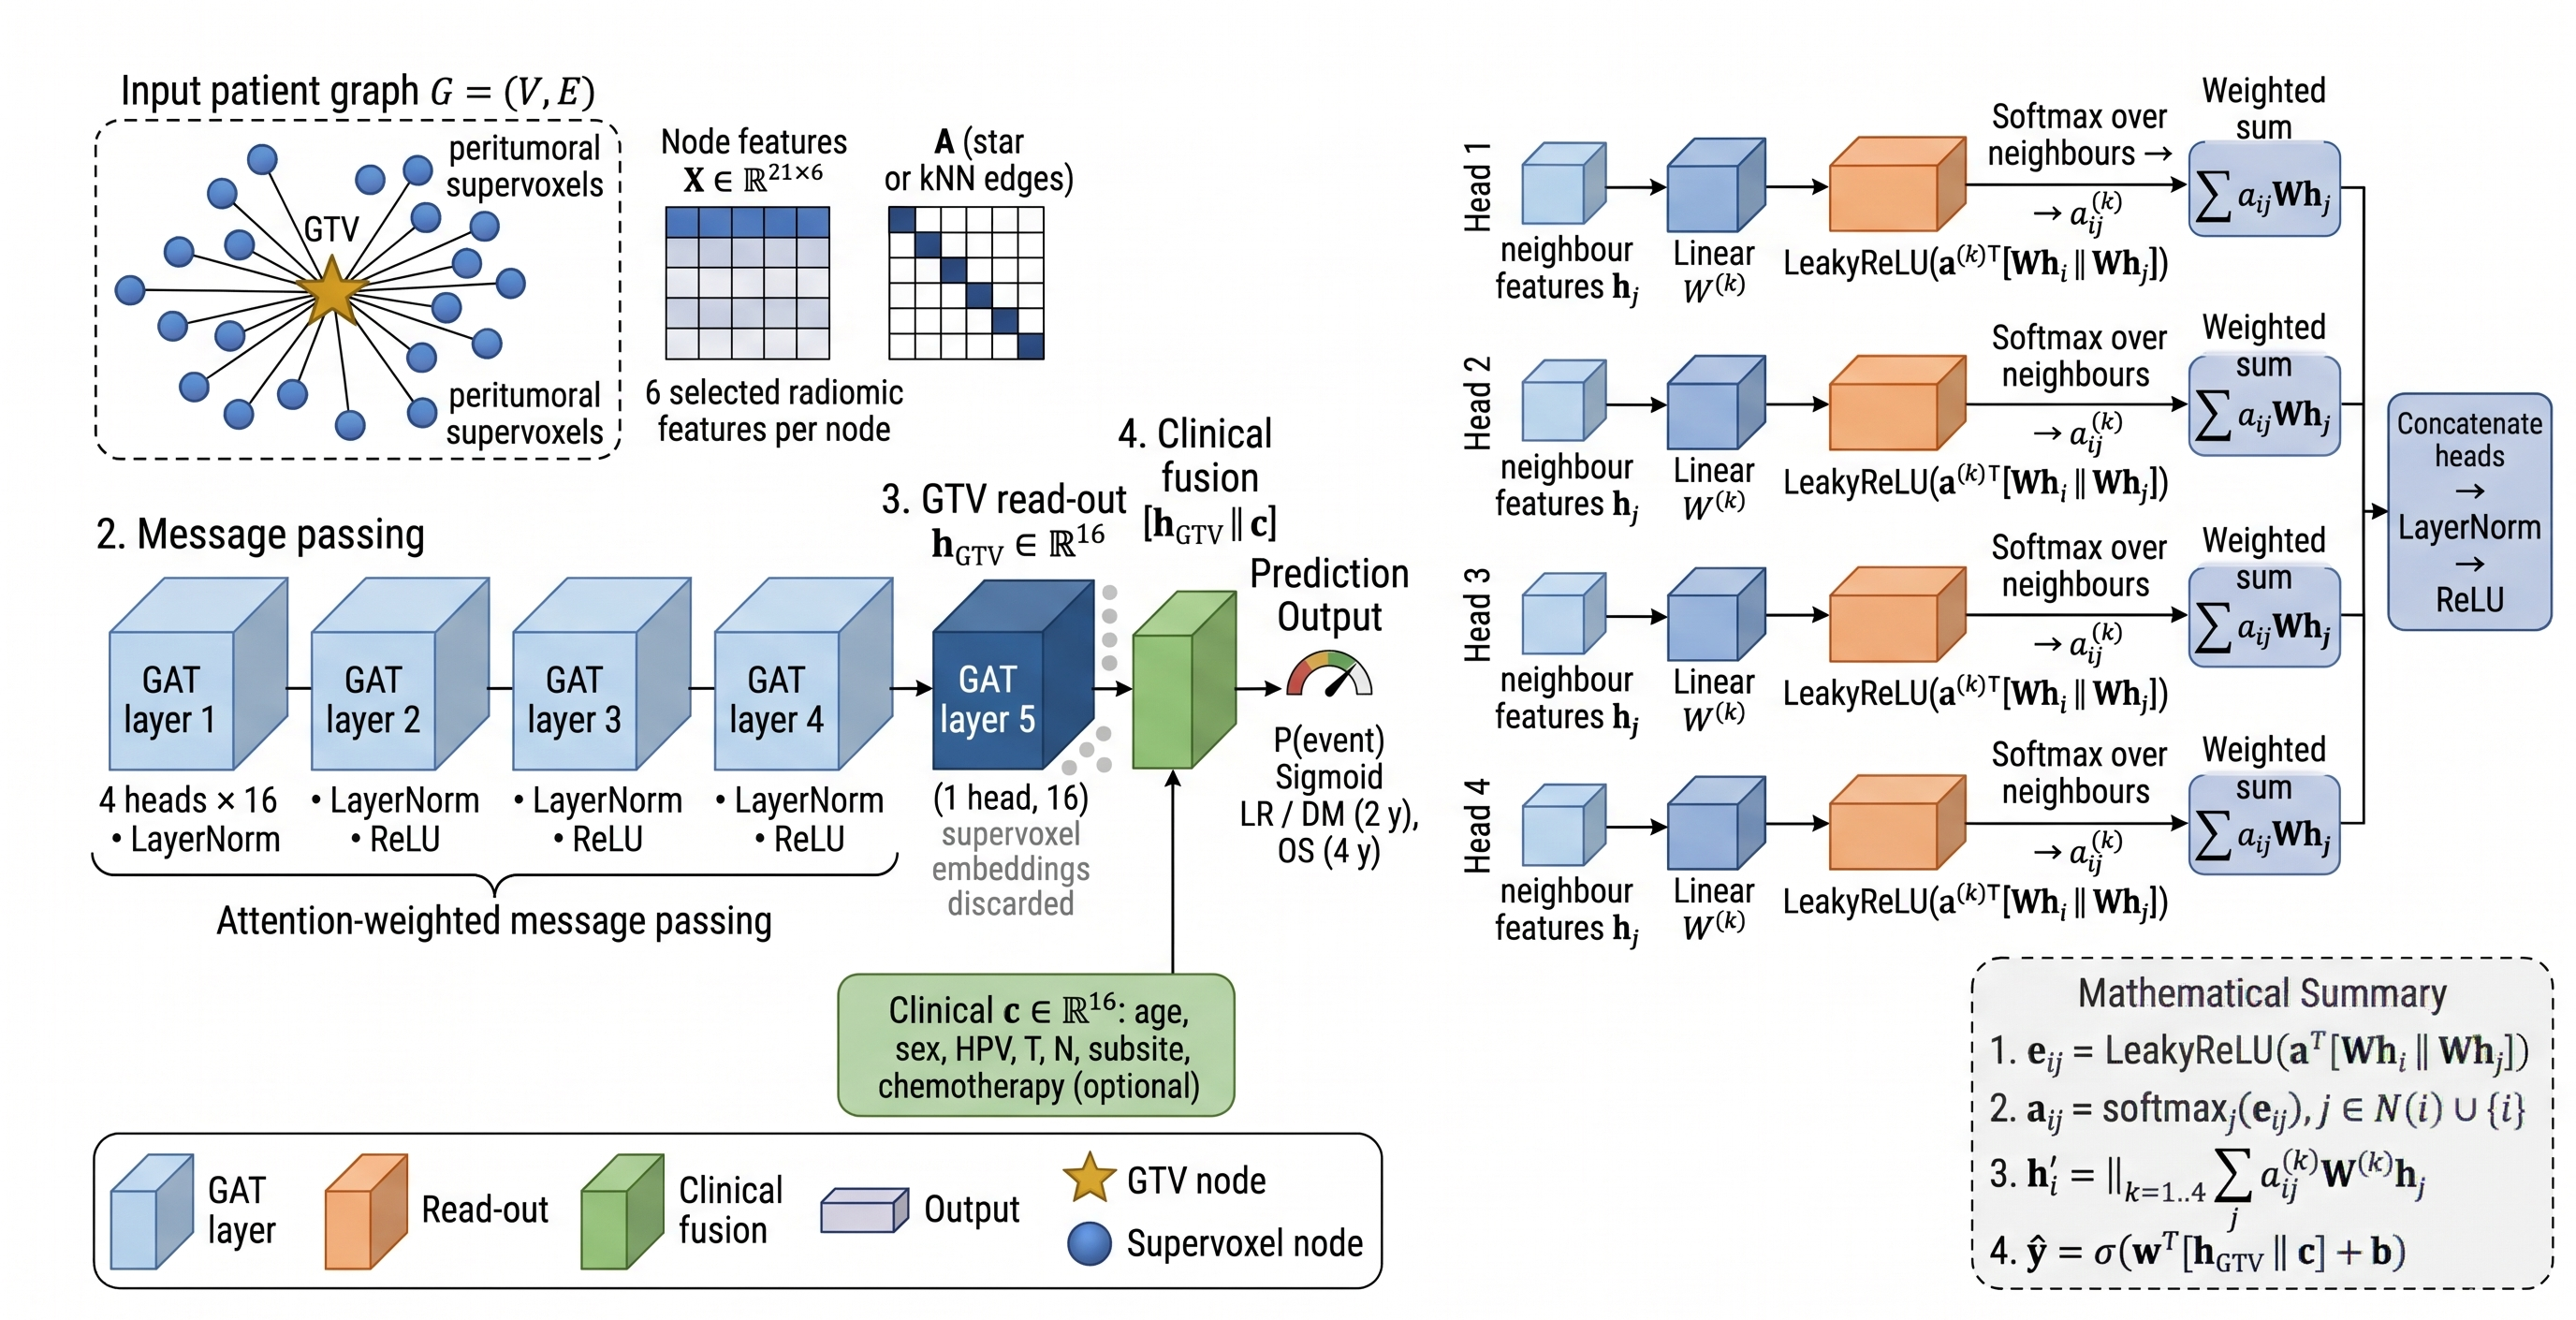
\includegraphics[width=\textwidth]{fig_architecture_author.png}
\caption{Radiomic graph attention network. \textbf{Left:} each patient is represented as a graph of the gross tumour volume (GTV, star) and 20 peritumoral supervoxels, each described by six selected radiomic features and connected by star or kNN edges. Five GAT layers perform attention-weighted message passing; the embedding of the GTV node is read out, optionally fused with 16 clinical variables, and mapped by a linear layer and sigmoid to the probability of the event (LR or DM within 2 years, death within 4 years). \textbf{Right:} multi-head graph attention at the GTV node. Each of four heads transforms the neighbour features, scores every edge, normalises the scores over the neighbourhood and forms a weighted sum; the heads are concatenated and followed by layer normalisation and ReLU. The LR/OS configuration is shown; the DM network has three layers and eight units per head.}\label{fig:arch}
\end{figure}

\subsection{Patient cohorts and endpoints}
The development cohort was drawn from the Head-Neck-PET-CT collection~\cite{vallieres2017tcia,vallieres2017}, which comprises \nHNPETclin{} patients with histologically confirmed HNSCC treated with radiotherapy, with or without chemotherapy, at four centres in Qu\'ebec, Canada: Centre hospitalier de l'Universit\'e de Montr\'eal (CHUM), Centre hospitalier universitaire de Sherbrooke (CHUS), H\^opital g\'en\'eral juif (HGJ) and H\^opital Maisonneuve-Rosemont (HMR). Outcomes and their timing were taken from the collection's clinical spreadsheet (version 2, May 2018). A CT volume with a delineated primary GTV was available for \nHNPETimg{} of these patients (CHUM \nCHUM, CHUS \nCHUS, HGJ \nHGJ, HMR \nHMR). The external test cohort was the HN1 collection~\cite{wee2019hn1,aerts2014} of 137 patients with oropharyngeal or laryngeal cancer treated at MAASTRO Clinic, Maastricht, the Netherlands. This cohort was never used for selection, scaling, training or model choice. Both collections are distributed by The Cancer Imaging Archive~\cite{clark2013tcia}; the original studies obtained institutional approval, and no further approval was required for this secondary analysis.

Following Mateus et al.~\cite{mateus2023}, LR and DM were defined as an event within two years of diagnosis and OS as death from any cause within four years, the median follow-up of the development data. Patients without an event who were followed for less than the horizon were excluded from the analysis of that endpoint, and events occurring after the horizon were counted as negative. The resulting cohorts are described in Table~\ref{tab:cohort}.

\begin{table}[!htb]
\caption{Patient characteristics and outcome cohorts.}\label{tab:cohort}
\centering\small
\begin{tabular}{@{}lll@{}}
\toprule
Characteristic & Canadian centres$^{a}$ & MAASTRO (HN1) \\
 & training / validation & external test \\
\midrule
Patients with CT and GTV & 199 & 137 \\
Age, median (IQR), y & 63 (57--70) & 61 (56--67) \\
Male sex & 147 (74\%) & 111 (81\%) \\
HPV positive & 74 (37\%) & 23 (17\%) \\
HPV negative & 19 (10\%) & 58 (42\%) \\
HPV unknown & 106 (53\%) & 56 (41\%) \\
Oropharynx & 199 (100\%) & 88 (64\%) \\
Larynx & 0 (0\%) & 49 (36\%) \\
Other subsite & 0 (0\%) & 0 (0\%) \\
T3--T4 & 84 (42\%) & 70 (51\%) \\
N2--N3 & 150 (75\%) & 61 (45\%) \\
Concurrent chemotherapy & 173 (87\%) & 37 (27\%) \\
\midrule
\multicolumn{3}{@{}l}{\textit{Outcome cohorts$^{b}$, patients (events, rate)}} \\
LR: analysed (events) & 190 (13, 6.8\%) & 121 (30, 24.8\%) \\
DM: analysed (events) & 191 (12, 6.3\%) & 109 (7, 6.4\%) \\
OS: analysed (events) & 92 (19, 20.7\%) & 135 (45, 33.3\%) \\
\botrule
\end{tabular}

\tabnote{IQR, interquartile range; HPV, human papillomavirus; LR, locoregional recurrence; DM, distant metastasis; OS, overall survival. $^{a}$Head-Neck-PET-CT patients (CHUM, CHUS, HGJ, HMR) with CT and primary GTV. $^{b}$Patients eligible for each endpoint, that is, with an event within the horizon (2 years for LR and DM, 4 years for OS) or event-free follow-up of at least the horizon.}
\end{table}

\subsection{Model development and validation strategy}
Two development designs were used, both with MAASTRO as the external test set~\cite{mateus2023}. In the 5-fold cross-validation design, the Canadian patients were partitioned into five folds stratified by outcome, and the complete pipeline, from feature selection to model training, was refitted on four folds and validated on the fifth. Configurations were compared on the pooled out-of-fold validation AUC, in which every patient is validated exactly once, and external predictions were averaged over the five fold models. Because Mateus et al.\ reported the mean and range of the per-fold test AUCs, these were also recorded for direct comparison. In the cohort-split design of Diamant et al.~\cite{diamant2019}, models were trained on HGJ and CHUS and validated on HMR and CHUM, so that validation also measured transfer between institutions.

\subsection{Image preprocessing and radiomic feature extraction}
CT volumes were resampled to 1\,mm isotropic voxels with linear interpolation and the GTV masks to the same grid with nearest-neighbour interpolation. The volume was cropped to a box extending 50\,mm beyond the GTV in every direction, which defines the peritumoral region~\cite{bae2025radgraph}. GTV voxels were removed from this region, intensities were normalised to $[0,1]$ inside it, and the region was divided into approximately 100 supervoxels by zero-parameter simple linear iterative clustering (SLIC-zero)~\cite{achanta2012slic} with enforced connectivity; supervoxels of fewer than 8 voxels were discarded. For the GTV and every supervoxel, 93 features were extracted with PyRadiomics~\cite{vangriethuysen2017} using a fixed bin width of 25\,HU: 18 first-order features and 24 grey-level co-occurrence (GLCM), 16 run-length (GLRLM), 16 size-zone (GLSZM), 14 dependence (GLDM) and 5 neighbourhood grey-tone difference (NGTDM) features. Shape features were excluded because they describe the supervoxel construction rather than the tissue~\cite{bae2025radgraph}.

\subsection{Feature selection}
Selectors were applied to the GTV features of the training patients after removal of near-constant features, a signed logarithmic transform of heavy-tailed features (absolute skewness above 2) and z-scoring. To compare strategies at equal model capacity, every data-driven selector retained $k=6$ features.

Two non-adaptive strategies served as references. The first was the fixed endpoint-specific feature set of RadGraph (four features for LR and six for DM, Table~S3 of the original work)~\cite{bae2025radgraph}; because no OS set was published, mRMR acted as the OS reference. The second used all 93 features without selection. Four established supervised selectors were compared: mRMR~\cite{peng2005mrmr}, which greedily maximises the ratio of relevance (ANOVA $F$) to redundancy (mean absolute correlation with features already selected); L1-penalised logistic regression (LASSO)~\cite{tibshirani1996lasso} with the penalty chosen by inner cross-validated AUC and features ranked by their entry point along the regularisation path; Boruta~\cite{kursa2010boruta}, which tests random-forest importance against permuted shadow features; and recursive feature elimination with a random forest (RFE-RF)~\cite{guyon2002rfe}.

Graph-FS~\cite{moradmand2025graphfs} builds a feature graph in which two features are connected if their absolute Pearson correlation exceeds $\bar r+\alpha s_r$, where $\bar r$ and $s_r$ are the mean and standard deviation of all pairwise absolute correlations and $\alpha=0.3$; isolated features are linked to their most correlated partner. In the connected-component variant (Graph-FS CC), one representative with the highest degree centrality is kept per component. Because the 93 features formed a single component at $\alpha=0.3$, $\alpha$ was increased in steps of 0.1 until at least $k$ components existed. In the spectral variant~\cite{vonluxburg2007spectral}, the features are clustered by $k$-means on the eigenvectors of the unnormalised graph Laplacian associated with the $k$ smallest eigenvalues, and the feature closest to each cluster centroid is kept. Both variants are label-free: they control redundancy but ignore the outcome. A hybrid variant was therefore introduced, in which the feature graph is partitioned into $\max(2k,\text{eigengap})$ spectral communities, the most outcome-relevant feature (largest ANOVA $F$) of each community is taken as its representative, and the $k$ most relevant representatives are retained. Redundancy is thus controlled by the label-free graph, while relevance is determined by the outcome. The complete procedure is illustrated on the training data of the first cross-validation fold in Fig.~\ref{fig:gfs}, and algorithmic details are given in Supplementary Section~4.

\begin{figure}[!htb]
\centering
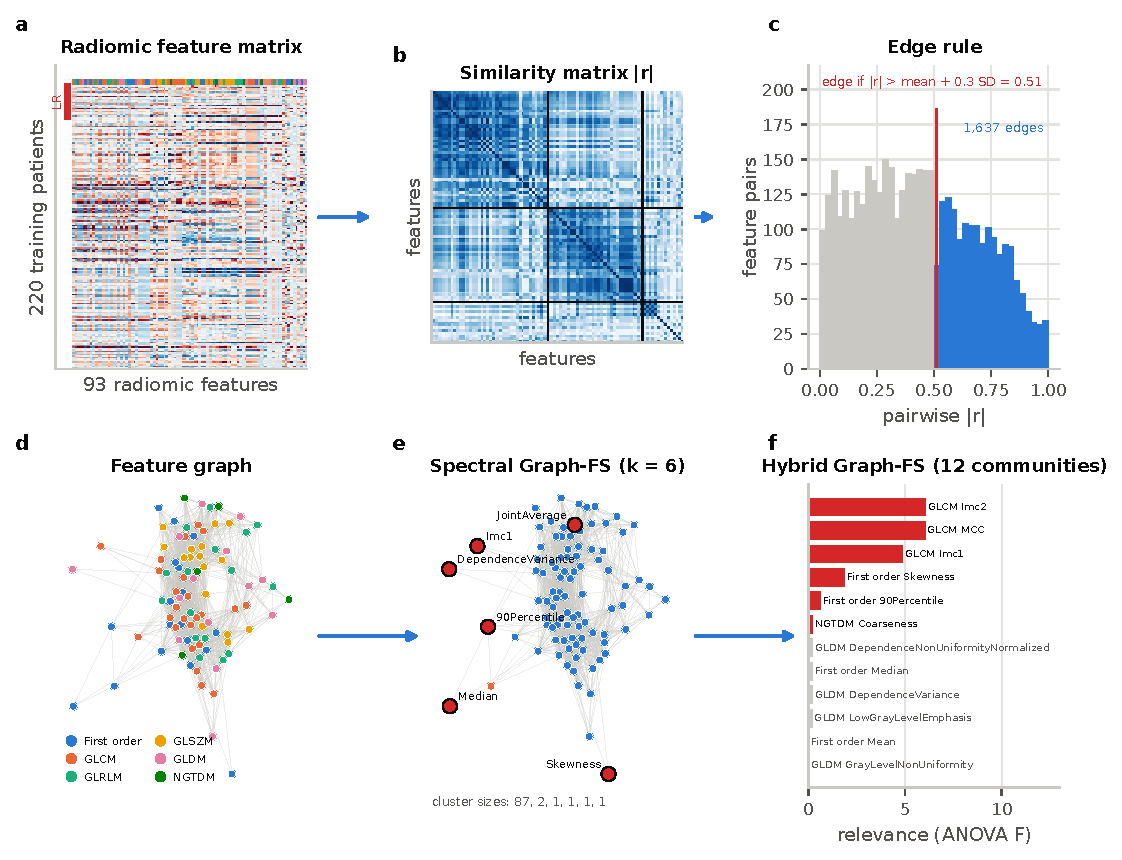
\includegraphics[width=\textwidth]{fig_graphfs_workflow.pdf}
\caption{Graph-based feature selection, illustrated on the training data of the first cross-validation fold for locoregional recurrence (\gfsTrainN{} patients, \gfsTrainEv{} events). \textbf{a}~z-scored matrix of the 93 GTV radiomic features (columns, coloured strip: feature class) of the training patients (rows; red bar: patients with locoregional recurrence). \textbf{b}~Absolute Pearson correlation matrix, ordered by feature community; black lines delimit the two largest communities. \textbf{c}~Distribution of pairwise absolute correlations; feature pairs above the threshold of mean + 0.3 standard deviations (\gfsThr) form the \gfsEdges{} edges of the feature graph. \textbf{d}~Resulting feature graph, nodes coloured by feature class. \textbf{e}~Spectral Graph-FS partitions the graph into $k=6$ clusters (sizes in the panel) and selects the feature closest to each cluster centroid (red); because \gfsBigCluster{} of the 93 features form a single cluster, five representatives are structurally isolated features. \textbf{f}~Hybrid Graph-FS partitions the same graph into \gfsHybComm{} communities, takes the most outcome-relevant feature (ANOVA $F$) of each community as its representative, and retains the six most relevant representatives (red).}\label{fig:gfs}
\end{figure}

\subsection{Graph construction}
Each patient graph contained the GTV, which served as the read-out node, and $K=20$ supervoxel nodes. Node features were the selected features, z-scored with the means and standard deviations of the GTV features of the training patients, as in the RadGraph implementation, and clipped at $\pm5$. Four topologies were compared (Fig.~\ref{fig:topo}). The radiomic star of RadGraph connects the GTV with the $K$ supervoxels that are closest to it in the selected-feature space, whereas the spatial star connects it with the $K$ supervoxels closest to its centroid in physical space. The two kNN topologies retain the corresponding star and add undirected edges between every node and its four nearest neighbours, in feature space (radiomic kNN) or physical space (spatial kNN), so that information can also be exchanged between supervoxels.

\begin{figure}[!htb]
\centering
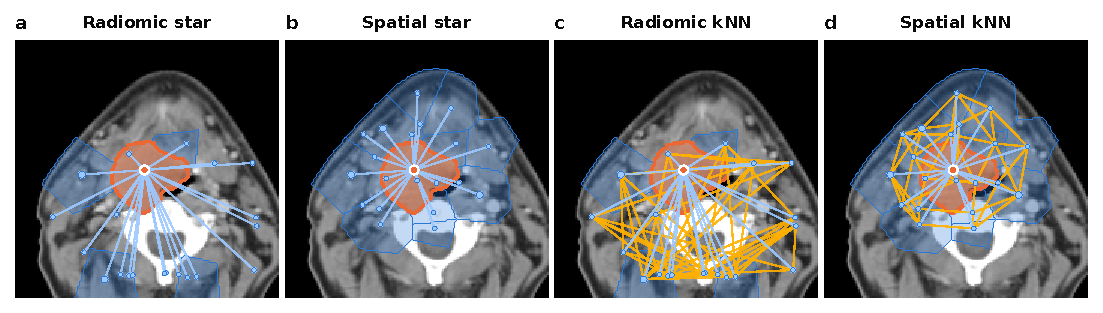
\includegraphics[width=\textwidth]{fig2_topologies.pdf}
\caption{The four graph topologies on the planning CT of an external test patient (\topoPid, oropharyngeal cancer; axial slice through the GTV centroid, soft-tissue window). The GTV is shown in orange with its centroid as the read-out node; the 20 selected supervoxels are outlined in blue where they intersect the slice, and edges are projected onto the slice. \textbf{a}~Radiomic star (RadGraph): supervoxels most similar to the GTV in feature space, which may lie far from the tumour. \textbf{b}~Spatial star: the supervoxels nearest to the GTV. \textbf{c}~Radiomic kNN and \textbf{d}~spatial kNN add edges (yellow) between each node and its four nearest neighbours in feature space and physical space, respectively. Graphs are those used by the models of the first cross-validation fold with the RadGraph features.}\label{fig:topo}
\end{figure}

\subsection{Graph attention network}
The network reproduced the RadGraph architecture and its endpoint-specific hyper-parameters (Fig.~\ref{fig:arch}; Supplementary Table~S3)~\cite{bae2025radgraph}. For LR, four GAT layers~\cite{velickovic2018gat} with four attention heads of 16 units, each followed by graph-wise layer normalisation and a ReLU, precede a final single-head layer. The 16-dimensional embedding of the GTV node is read out, passed through dropout and, when clinical data were used, concatenated with the 16 encoded clinical variables before a linear output layer. The DM model has three layers with eight units per head and stronger dropout. Because RadGraph did not specify an OS model, OS used the LR settings. The LR network with clinical input has 15,057 trainable parameters and the DM network 1,841.

Training used binary cross-entropy with per-epoch class resampling (both classes resampled to the mean class size for LR and OS, minority oversampling for DM), the Adam optimiser with a linear warm-up, learning-rate reduction on a validation-loss plateau, gradient clipping and early stopping with a patience of 50 epochs. The checkpoint with the lowest validation loss was retained, as in RadGraph. As a sensitivity analysis, the checkpoint rule of Mateus et al.\ was also applied, which selects the epoch with the highest validation AUC among epochs whose training--validation AUC gap does not exceed 0.05, relaxing the threshold in steps of 0.05 until an epoch qualifies~\cite{mateus2023}. Every configuration was trained with three random seeds and the predicted probabilities were averaged. The implementation used PyTorch~\cite{paszke2019pytorch} and PyTorch Geometric~\cite{fey2019pyg}.

\subsection{Clinical variables and comparator models}
Clinical variables recorded identically in both cohorts were used: age, sex, HPV status (positive, negative or unknown), T and N category, subsite (oropharynx or larynx) and concurrent chemotherapy. They were one-hot encoded, and age was scaled with the training range. Two random-forest baselines~\cite{breiman2001rf,pedregosa2011sklearn} were trained on the same splits. The first used the GTV features chosen by each selector, so that its comparison with the GAT isolates the contribution of the peritumoral graph. The second used the clinical variables alone.

\subsection{Statistical analysis}
Discrimination was measured by the area under the receiver operating characteristic curve (AUC) with 95\% percentile bootstrap confidence intervals based on 1000 resamples~\cite{efron1993}. Within each endpoint, design and input set, every configuration was compared with the reference configuration (RadGraph features with the radiomic star for LR and DM, mRMR with the radiomic star for OS) and with the random forest on the same features using paired DeLong tests~\cite{delong1988}, with Holm correction across configurations~\cite{holm1979}. Selection stability was quantified with the Kuncheva consistency index~\cite{kuncheva2007}, which corrects the overlap of equally sized subsets for chance, complemented by the Jaccard index and Kendall's coefficient of concordance~\cite{kendall1939}. Stability was evaluated across the five CV folds, across 30 bootstrap resamples of the training data within each fold, and between selections made separately in the two largest centres (CHUS and HGJ), the last requiring at least 15 patients and three events per centre. Associations between stability and external AUC across selectors, and between validation and external AUC across configurations, were summarised with Spearman's $\rho$.

\subsection{Implementation}
All pipeline stages are cached and deterministic for a given seed. Each trained model is stored as a self-contained checkpoint that includes the network weights, hyper-parameters, the selected features, the training scaler, the clinical encoder, the decision threshold and the topology, and a command-line tool applies the stored ensembles to new patients supplied as CT and GTV images without retraining. Re-applying the stored models reproduced the reported external predictions to within $10^{-7}$.

%% =========================================================================================
\section{Results}\label{sec:results}

\subsection{Patient characteristics}
The development cohort of \nHNPETimg{} patients was entirely oropharyngeal, whereas 36\% of the MAASTRO patients had laryngeal cancer (Table~\ref{tab:cohort}). HPV status was unknown for about half of the Canadian patients, HPV-positive disease was more frequent in the development than in the test cohort, and concurrent chemotherapy was given to most Canadian but a minority of Dutch patients. Events were scarce in the development data, with \eLRHNPET{} LR events among \nLRHNPET{} patients, \eDMHNPET{} DM events among \nDMHNPET{} patients and \eOSHNPET{} deaths among \nOSHNPET{} patients, so that each CV validation fold contained only two or three LR or DM events. The external cohort contained \eLRMAASTRO{} LR, \eDMMAASTRO{} DM and \eOSMAASTRO{} OS events. The clinical file lists \allEvLR{} LR, \allEvDM{} DM and \allEvOS{} OS events among all eligible Canadian patients; the patients without available images therefore carried more than half of the events (Supplementary Table~S1).

\draftnote{All Canadian patients with images are oropharyngeal, which suggests that the local image folder is the HECKTOR subset~\cite{oreiller2022hecktor} of Head-Neck-PET-CT. In that case the CT and GTVs may be HECKTOR re-annotations of the PET/CT CT rather than the planning-CT contours used by Mateus et al. Confirm the image source and describe it here.}

\subsection{External validation performance}
External performance of the configuration chosen on validation, of the RadGraph reference and of the baselines is summarised in Table~\ref{tab:main}; the receiver operating characteristic curves of all endpoints are shown in Fig.~\ref{fig:roc} and the confidence intervals are compared in Fig.~\ref{fig:overview}. For LR, the configuration chosen in the cohort split reached an AUC of \aucLRCohImgChosen{} (95\% CI \ciLRCohImgChosen) with imaging alone and \aucLRCohClinChosen{} (\ciLRCohClinChosen) with clinical variables, compared with \aucLRCohImgRef{} and \aucLRCohClinRef{} for the reference configuration and \aucLRCohClinClinRF{} for the clinical-only random forest. In cross-validation the fold-ensemble AUCs of the chosen configurations were \aucLRCVImgChosen{} (\ciLRCVImgChosen) and \aucLRCVClinChosen{} (\ciLRCVClinChosen). Here the reference was numerically the stronger GAT, reaching \aucLRCVImgRef{} and \aucLRCVClinRef, while the clinical-only forest reached \aucLRCVClinClinRF. None of the \nConfigLR{} LR configurations differed significantly from the reference after Holm correction.

\begin{table}[!htb]
\caption{External test performance (MAASTRO) of the configuration chosen on validation AUC, the RadGraph reference configuration, the best random forest on selected GTV features and a clinical-only random forest (primary checkpoint rule).}\label{tab:main}
\centering
\resizebox{\textwidth}{!}{\begin{tabular}{@{}llllcc@{}}
\toprule
Outcome / design & Inputs & Model & Configuration & Val. AUC & Test AUC [95\% CI] \\
\midrule
LR, 5-fold CV & Img & GAT, chosen on validation & Boruta + Radiomic kNN & 0.71 & 0.61 [0.50, 0.72]$^{p=1.00}$ \\
 & Img & GAT, reference & Table S3 (RadGraph) + Radiomic star & 0.54 & 0.63 [0.51, 0.75] \\
 & Img & RF, selected GTV features & All features & 0.69 & 0.56 [0.45, 0.68] \\
 & Img+Clin & GAT, chosen on validation & All features + Radiomic kNN & 0.74 & 0.58 [0.46, 0.69]$^{p=1.00}$ \\
 & Img+Clin & GAT, reference & Table S3 (RadGraph) + Radiomic star & 0.51 & 0.69 [0.59, 0.80] \\
 & Img+Clin & RF, clinical only & -- & 0.71 & 0.66 [0.56, 0.76] \\
\addlinespace
LR, Cohort split & Img & GAT, chosen on validation & All features + Radiomic kNN & 0.75 & 0.63 [0.51, 0.75]$^{p=1.00}$ \\
 & Img & GAT, reference & Table S3 (RadGraph) + Radiomic star & 0.28 & 0.52 [0.41, 0.64] \\
 & Img & RF, selected GTV features & All features & 0.61 & 0.56 [0.44, 0.68] \\
 & Img+Clin & GAT, chosen on validation & Graph-FS (spectral) + Radiomic kNN & 0.80 & 0.71 [0.62, 0.81]$^{p=0.72}$ \\
 & Img+Clin & GAT, reference & Table S3 (RadGraph) + Radiomic star & 0.27 & 0.55 [0.43, 0.67] \\
 & Img+Clin & RF, clinical only & -- & 0.67 & 0.63 [0.52, 0.75] \\
\midrule
DM, 5-fold CV & Img & GAT, chosen on validation & All features + Radiomic kNN & 0.64 & 0.66 [0.49, 0.82]$^{p=0.24}$ \\
 & Img & GAT, reference & Table S3 (RadGraph) + Radiomic star & 0.60 & 0.41 [0.24, 0.58] \\
 & Img & RF, selected GTV features & Graph-FS (hybrid) & 0.82 & 0.58 [0.34, 0.79] \\
 & Img+Clin & GAT, chosen on validation & All features + Radiomic kNN & 0.56 & 0.65 [0.44, 0.85]$^{p=1.00}$ \\
 & Img+Clin & GAT, reference & Table S3 (RadGraph) + Radiomic star & 0.38 & 0.60 [0.32, 0.85] \\
 & Img+Clin & RF, clinical only & -- & 0.63 & 0.80 [0.70, 0.89] \\
\addlinespace
DM, Cohort split & Img & GAT, chosen on validation & RFE-RF + Spatial star & 0.81 & 0.36 [0.14, 0.60]$^{p=1.00}$ \\
 & Img & GAT, reference & Table S3 (RadGraph) + Radiomic star & 0.68 & 0.40 [0.22, 0.56] \\
 & Img & RF, selected GTV features & Graph-FS (CC) & 0.73 & 0.60 [0.43, 0.77] \\
 & Img+Clin & GAT, chosen on validation & All features + Radiomic star & 0.75 & 0.19 [0.10, 0.31]$^{p<0.01}$ \\
 & Img+Clin & GAT, reference & Table S3 (RadGraph) + Radiomic star & 0.49 & 0.68 [0.44, 0.87] \\
 & Img+Clin & RF, clinical only & -- & 0.54 & 0.70 [0.57, 0.81] \\
\midrule
OS, 5-fold CV & Img & GAT, chosen on validation & Graph-FS (spectral) + Spatial kNN & 0.69 & 0.46 [0.35, 0.56]$^{p=0.20}$ \\
 & Img & GAT, reference & mRMR + Radiomic star & 0.57 & 0.62 [0.52, 0.72] \\
 & Img & RF, selected GTV features & Graph-FS (spectral) & 0.69 & 0.52 [0.41, 0.62] \\
 & Img+Clin & GAT, chosen on validation & Graph-FS (spectral) + Spatial kNN & 0.69 & 0.47 [0.36, 0.57]$^{p=0.11}$ \\
 & Img+Clin & GAT, reference & mRMR + Radiomic star & 0.59 & 0.66 [0.56, 0.75] \\
 & Img+Clin & RF, clinical only & -- & 0.66 & 0.60 [0.51, 0.69] \\
\addlinespace
OS, Cohort split & Img & GAT, chosen on validation & Graph-FS (spectral) + Spatial kNN & 0.73 & 0.45 [0.35, 0.56]$^{p=1.00}$ \\
 & Img & GAT, reference & mRMR + Radiomic star & 0.55 & 0.56 [0.46, 0.66] \\
 & Img & RF, selected GTV features & Graph-FS (spectral) & 0.66 & 0.52 [0.42, 0.63] \\
 & Img+Clin & GAT, chosen on validation & Graph-FS (spectral) + Spatial kNN & 0.73 & 0.48 [0.37, 0.57]$^{p=0.56}$ \\
 & Img+Clin & GAT, reference & mRMR + Radiomic star & 0.55 & 0.62 [0.52, 0.73] \\
 & Img+Clin & RF, clinical only & -- & 0.69 & 0.42 [0.32, 0.53] \\
\botrule
\end{tabular}
}
\tabnote{Img, imaging only; Img+Clin, imaging and clinical variables; Val.\ AUC, pooled out-of-fold (CV) or validation-cohort (cohort split) AUC on which the configuration was chosen; Test AUC, fold- and seed-ensemble AUC with 95\% bootstrap CI; superscript $p$, Holm-corrected DeLong test against the reference. Reference: RadGraph Table S3 features with radiomic star (LR, DM) or mRMR with radiomic star (OS).}
\end{table}

\begin{figure}[!htb]
\centering
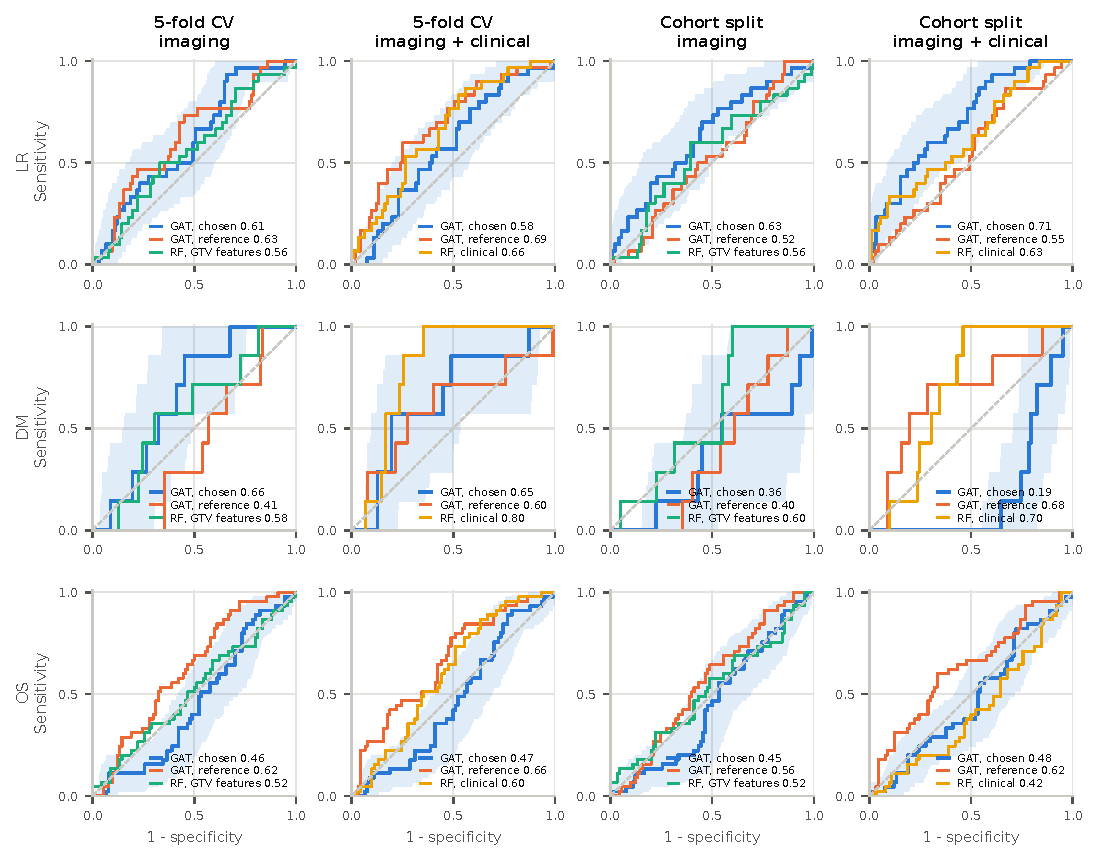
\includegraphics[width=\textwidth]{fig_roc_all.pdf}
\caption{External ROC curves on MAASTRO for locoregional recurrence (top, \nLRMAASTRO{} patients, \eLRMAASTRO{} events), distant metastasis (middle, \nDMMAASTRO{} patients, \eDMMAASTRO{} events) and overall survival (bottom, \nOSMAASTRO{} patients, \eOSMAASTRO{} deaths). Columns show the two validation designs with imaging only and with imaging and clinical variables. Each panel compares the GAT configuration chosen on validation (shaded: 95\% bootstrap band), the RadGraph reference configuration and a random forest on the selected GTV features or on clinical variables; legend values are external AUCs.}\label{fig:roc}
\end{figure}

For DM, with only \eDMMAASTRO{} external events, the confidence intervals spanned most of the AUC range, and configurations chosen on validation ranged from \aucDMCohClinChosen{} to \aucDMCVImgChosen. All \nSigDM{} DM configurations that differed significantly from the reference performed worse than it. The clinical-only random forest was the strongest DM model, with an AUC of \aucDMCVClinClinRF{} (\ciDMCVClinClinRF) in cross-validation. For OS, the configurations chosen on validation reached \aucOSCohImgChosen--\aucOSCohClinChosen{} in both designs, whereas the pre-specified mRMR reference reached \aucOSCVImgRef{} (\ciOSCVImgRef) with imaging alone and \aucOSCVClinRef{} (\ciOSCVClinRef) with clinical variables in cross-validation.

\begin{figure}[!htb]
\centering
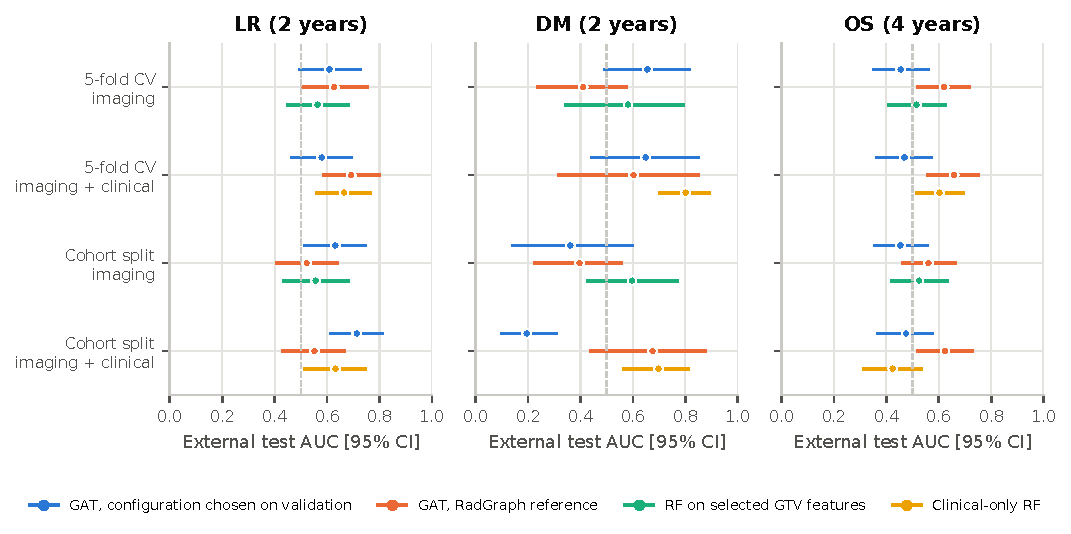
\includegraphics[width=\textwidth]{fig5_auc_overview.pdf}
\caption{External test AUC with 95\% bootstrap CI for all endpoints, validation designs and input sets. The dashed line marks chance discrimination.}\label{fig:overview}
\end{figure}

Across the entire grid, external LR AUCs ranged from \gridMinLR{} to \gridMaxLR{} (median \gridMedLR), and \gridAboveLR\% of the LR configurations exceeded 0.5, whereas the corresponding medians were \gridMedDM{} for DM and \gridMedOS{} for OS. LR was therefore the only endpoint for which the radiomic graph carried a consistent, if modest, signal.

\subsection{Comparison with a convolutional neural network benchmark}
Table~\ref{tab:mateus} places the chosen GATs next to the convolutional neural network of Mateus et al., which was developed and tested on the same collections with the same designs~\cite{mateus2023}. For LR in the cohort split, the GAT exceeded the published network both with imaging alone (\aucLRCohImgChosen{} versus 0.45) and with clinical variables (\aucLRCohClinChosen{} versus 0.59), and in cross-validation the mean per-fold AUCs were similar (\foldLRImg{} versus 0.53 and \foldLRClin{} versus 0.57). For DM and OS the GAT was clearly inferior. Because the development data of the present study contained fewer than half of the events available to the published network and only oropharyngeal tumours, this comparison is indicative rather than conclusive.

\begin{table}[!htb]
\caption{External AUC on MAASTRO compared with the convolutional neural network of Mateus et al.~\cite{mateus2023}.}\label{tab:mateus}
\centering\small
\begin{tabular}{@{}lllll@{}}
\toprule
Outcome & Design & Inputs & This study (GAT) & Mateus et al.\ CNN \\
\midrule
Locoregional recurrence (2 y) & 5-fold CV & Img & 0.51 (0.41--0.62) & 0.53 (0.48--0.59) \\
 & 5-fold CV & Img+Clin & 0.56 (0.53--0.63) & 0.57 (0.53--0.60) \\
 & Cohort split & Img & 0.63 [0.51, 0.75] & 0.45 [0.32, 0.57] \\
 & Cohort split & Img+Clin & 0.71 [0.62, 0.81] & 0.59 [0.47, 0.70] \\
\midrule
Distant metastasis (2 y) & 5-fold CV & Img & 0.59 (0.38--0.76) & 0.83 (0.76--0.90) \\
 & 5-fold CV & Img+Clin & 0.50 (0.20--0.76) & 0.88 (0.86--0.90) \\
 & Cohort split & Img & 0.36 [0.14, 0.60] & 0.89 [0.79, 0.98] \\
 & Cohort split & Img+Clin & 0.19 [0.10, 0.31] & 0.93 [0.86, 0.99] \\
\midrule
Overall survival (4 y) & 5-fold CV & Img & 0.45 (0.42--0.49) & 0.63 (0.57--0.72) \\
 & 5-fold CV & Img+Clin & 0.48 (0.44--0.53) & 0.68 (0.63--0.71) \\
 & Cohort split & Img & 0.45 [0.35, 0.56] & 0.67 [0.57, 0.77] \\
 & Cohort split & Img+Clin & 0.48 [0.37, 0.57] & 0.69 [0.59, 0.79] \\
\botrule
\end{tabular}

\tabnote{5-fold CV: mean (range) of the five per-fold test AUCs, as reported by Mateus et al.; cohort split: AUC [95\% CI]. Values of Mateus et al.\ are taken from their Tables 3 (imaging) and 4 (network with clinical data). Their development set contained 297 Canadian patients, this study's \nHNPETimg.}
\end{table}

\subsection{Influence of feature selection, graph topology and clinical variables}
Mean external AUCs for every combination of selector and topology are shown in Fig.~\ref{fig:heatmap}. For LR, most combinations lay between 0.55 and 0.70, and the highest values were obtained with the RadGraph features and the hybrid Graph-FS, particularly with spatial topologies. Averaged over selectors, designs and input sets, the four topologies gave nearly identical LR AUCs (radiomic star \topoLRradiomicstar, spatial star \topoLRspatialstar, radiomic kNN \topoLRradiomicknn, spatial kNN \topoLRspatialknn). For OS, radiomic topologies tended to outperform spatial ones (\topoOSradiomicknn{} and \topoOSradiomicstar{} versus \topoOSspatialknn{} and \topoOSspatialstar), but no difference survived correction for multiple testing (Supplementary Tables~S5--S7). Adding clinical variables raised the mean external AUC for all three endpoints (LR from \meanImgLR{} to \meanClinLR, DM from \meanImgDM{} to \meanClinDM{} and OS from \meanImgOS{} to \meanClinOS).

\begin{figure}[!htb]
\centering
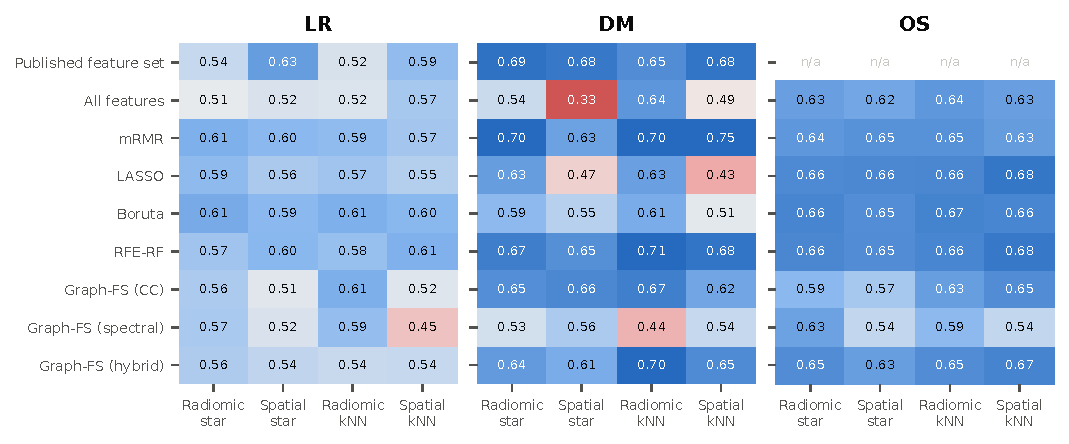
\includegraphics[width=\textwidth]{fig_heatmap.pdf}
\caption{Mean external AUC for each combination of feature-selection strategy (rows) and graph topology (columns), averaged over the two validation designs and the two input sets. Blue indicates AUC above and red below 0.5. No RadGraph feature set exists for OS (n/a).}\label{fig:heatmap}
\end{figure}

The contribution of the peritumoral graph was assessed by comparing each GAT with a random forest trained on exactly the same GTV features (Fig.~\ref{fig:gatrf}, Table~\ref{tab:gatrf}). For LR, the GAT achieved a higher mean external AUC than the corresponding forest for \gatRfLRCV{} feature sets in cross-validation and \gatRfLRCoh{} in the cohort split (mean AUC \gatMeanLRCV{} versus \rfMeanLRCV{} in cross-validation), although none of these differences was individually significant. For DM and OS the forests were generally at least as good as the GATs, with mean AUCs of \rfMeanDMCV{} versus \gatMeanDMCV{} for DM in cross-validation.

\begin{figure}[!htb]
\centering
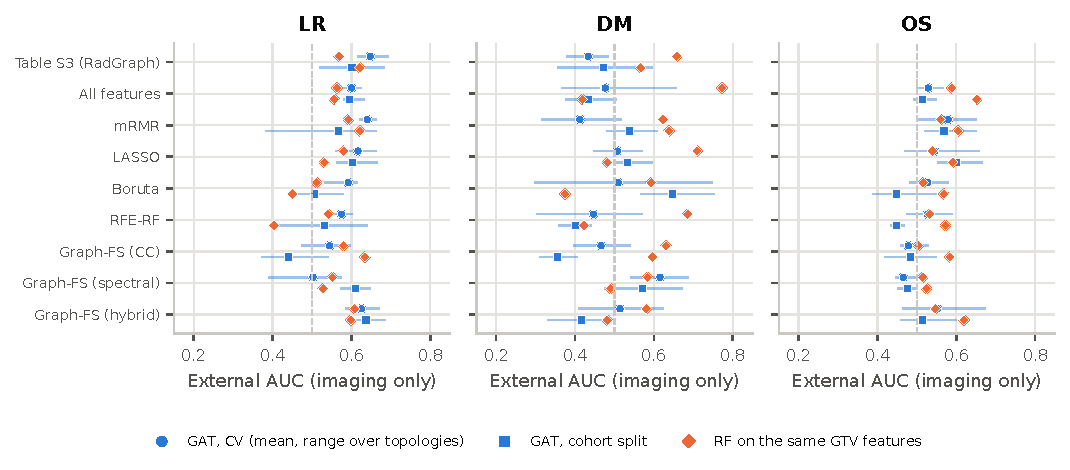
\includegraphics[width=\textwidth]{fig_gat_vs_rf.pdf}
\caption{Value of the peritumoral graph. For each selector, the external AUC of the GAT (mean and range over the four topologies, imaging only) is compared with a random forest trained on the same GTV features, for both validation designs.}\label{fig:gatrf}
\end{figure}

\begin{table}[!htb]
\caption{Graph attention network versus random forest on the same selected GTV features (imaging only).}\label{tab:gatrf}
\centering\small
\begin{tabular}{@{}llcccc@{}}
\toprule
Outcome & Design & GAT $>$ RF$^{a}$ & Mean AUC, GAT$^{b}$ & Mean AUC, RF & Significant$^{c}$ \\
\midrule
LR & 5-fold CV & 7/9 & 0.59 & 0.57 & 0 \\
 & Cohort split & 6/9 & 0.57 & 0.55 & 0 \\
\midrule
DM & 5-fold CV & 1/9 & 0.49 & 0.65 & 1 \\
 & Cohort split & 4/9 & 0.49 & 0.50 & 0 \\
\midrule
OS & 5-fold CV & 4/8 & 0.53 & 0.54 & 0 \\
 & Cohort split & 1/8 & 0.51 & 0.59 & 0 \\
\botrule
\end{tabular}

\tabnote{$^{a}$Number of feature sets (all strategies with a random-forest counterpart) for which the mean external AUC of the GAT over the four topologies exceeded that of the random forest. $^{b}$Mean over feature sets. $^{c}$Feature sets with at least one topology for which the GAT and the forest differed significantly (Holm-corrected DeLong test).}
\end{table}

\subsection{Feature selection stability}
The reproducibility of the selected features differed markedly between strategies (Table~\ref{tab:stability}, Fig.~\ref{fig:stability}). Across CV folds, spectral Graph-FS reached the highest Kuncheva index for LR (\kunSpecLR) and DM (\kunSpecDM) and the second highest for OS (\kunSpecOS, after Graph-FS CC with \kunCCOS), followed by the hybrid and CC variants. LASSO (\kunLassoLR{} for LR) and RFE-RF (\kunRfeLR) were the least stable. The same ordering was observed under bootstrap resampling, where spectral Graph-FS reached \bootSpecLR{} for LR. Selections made independently in two centres agreed poorly for every strategy, with Kuncheva indices of at most 0.21, again highest for spectral Graph-FS. Jaccard indices and Kendall's $W$ led to the same conclusions (Supplementary Table~S4).

\begin{table}[!htb]
\caption{Feature-selection stability (Kuncheva index; 1 indicates identical selections and 0 chance-level agreement). The highest value in each column is shown in bold.}\label{tab:stability}
\centering\small
\resizebox{\textwidth}{!}{\begin{tabular}{@{}lccccccccc@{}}
\toprule
 & \multicolumn{3}{c}{Across CV folds} & \multicolumn{3}{c}{Bootstrap} & \multicolumn{3}{c}{Across centres} \\
\cmidrule(lr){2-4}\cmidrule(lr){5-7}\cmidrule(lr){8-10}
Method & LR & DM & OS & LR & DM & OS & LR & DM & OS \\
\midrule
mRMR & 0.54 & 0.36 & 0.34 & 0.29 & 0.23 & 0.21 & 0.06 & 0.07 & -- \\
LASSO & 0.11 & 0.34 & 0.29 & 0.16 & 0.13 & 0.19 & 0.03 & 0.11 & -- \\
Boruta & 0.18 & 0.55 & 0.31 & 0.13 & 0.18 & 0.21 & 0.05 & 0.00 & -- \\
RFE-RF & 0.27 & 0.29 & 0.27 & 0.13 & 0.17 & 0.22 & 0.05 & 0.04 & -- \\
Graph-FS (CC) & 0.55 & 0.45 & \textbf{0.79} & 0.31 & 0.34 & 0.38 & 0.12 & 0.00 & -- \\
Graph-FS (spectral) & \textbf{0.64} & \textbf{0.73} & 0.63 & \textbf{0.55} & \textbf{0.54} & \textbf{0.43} & \textbf{0.21} & \textbf{0.18} & -- \\
Graph-FS (hybrid) & 0.59 & 0.70 & 0.43 & 0.38 & 0.34 & 0.29 & 0.11 & 0.11 & -- \\
\botrule
\end{tabular}
}
\tabnote{Across CV folds: mean pairwise index of the five fold-wise selections. Bootstrap: 30 resamples of the training data within each fold, averaged over folds. Across centres: selections made separately in CHUS and HGJ, averaged over folds; not estimable for OS because of fewer than three events per centre.}
\end{table}

\begin{figure}[!htb]
\centering
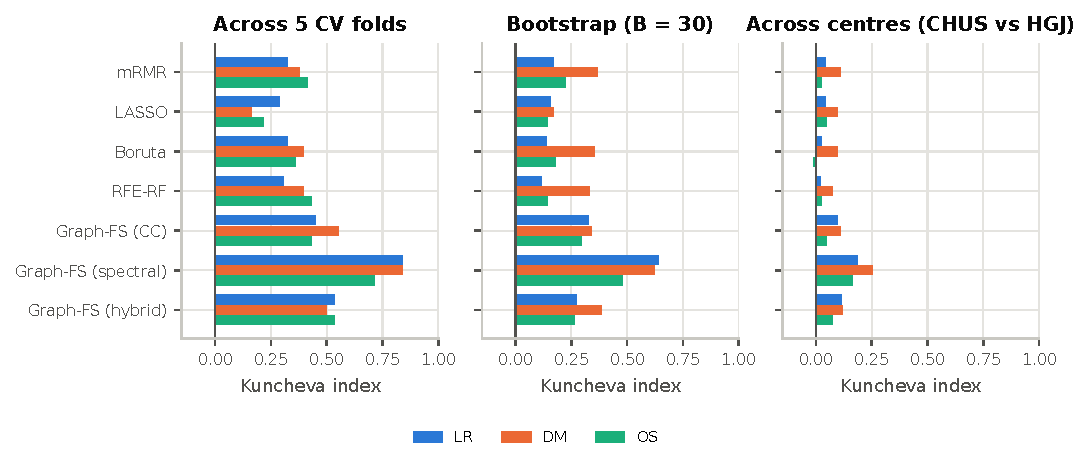
\includegraphics[width=\textwidth]{fig6_stability.pdf}
\caption{Feature-selection stability by strategy and endpoint in three settings. Graph-FS variants are the most stable across folds and bootstrap resamples, whereas selections transfer poorly between centres for all strategies.}\label{fig:stability}
\end{figure}

The origin of this stability is visible in the feature graph (Fig.~\ref{fig:gfs}b--e). At the Graph-FS threshold, almost all texture and first-order features formed one densely connected community, while a few features with distinctive correlation patterns, such as first-order skewness and median, GLCM informational measure of correlation and cluster shade, and GLDM dependence variance, formed communities of their own. Spectral Graph-FS selected GLCM informational measure of correlation, GLCM cluster shade and GLDM dependence variance in all five folds and first-order skewness in four (Fig.~\ref{fig:selfreq}). Several of these features, notably skewness and dependence variance, were also preferred by mRMR and the hybrid variant, whereas LASSO, Boruta and RFE-RF selected a different combination of correlated texture features in almost every fold.

\begin{figure}[!htb]
\centering
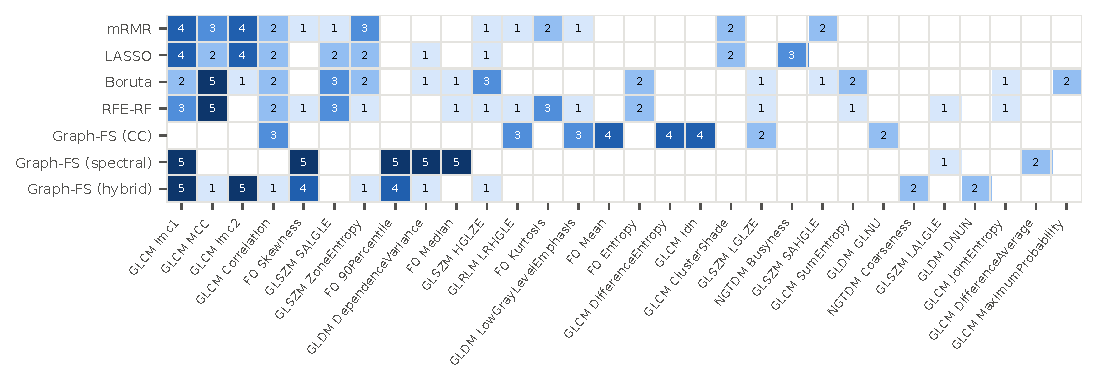
\includegraphics[width=\textwidth]{fig_selection_frequency.pdf}
\caption{Number of cross-validation folds (of five) in which each feature was selected by each strategy for locoregional recurrence, for the 30 most frequently selected features. FO, first order; long feature names are abbreviated by their initials (for example, SZNUN, size-zone non-uniformity normalised; SAHGLE, small-area high grey-level emphasis).}\label{fig:selfreq}
\end{figure}

\subsection{Stability, validation performance and external discrimination}
Stability did not translate into discrimination (Fig.~\ref{fig:stabauc}). Across selectors, the rank correlation between fold stability and mean external AUC was $\rho=\rhoStabLR$ for LR and $\rho=\rhoStabOS$ for OS; the positive value for DM ($\rho=\rhoStabDM$) rests on seven external events. For LR, mRMR and the hybrid Graph-FS combined intermediate-to-high stability (Kuncheva \kunMrmrLR{} and \kunHybLR) with the highest mean external AUCs, whereas the most stable strategy, spectral Graph-FS, was among the least discriminative.

\begin{figure}[!htb]
\centering
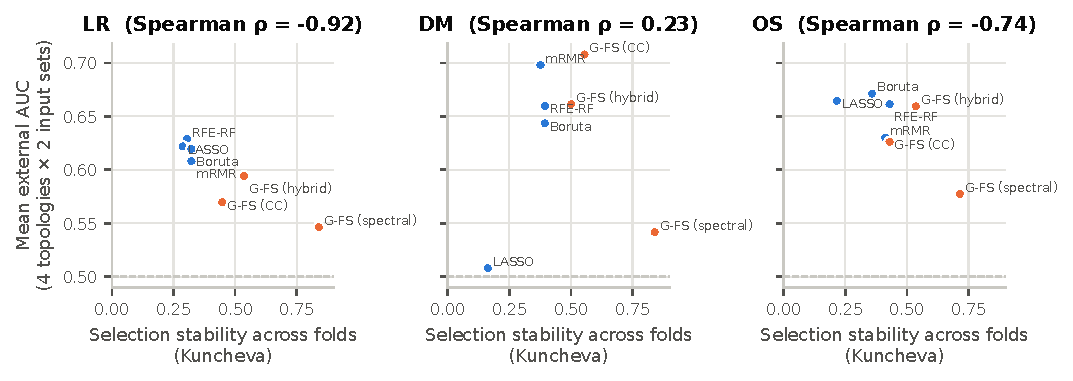
\includegraphics[width=\textwidth]{fig7_stability_vs_auc.pdf}
\caption{Selection stability across CV folds versus the mean external AUC of the GATs built on each selector (four topologies and two input sets, 5-fold CV). Graph-FS variants are shown in orange.}\label{fig:stabauc}
\end{figure}

Validation performance did not identify the configurations that generalised (Fig.~\ref{fig:valtest}). Across configurations, Spearman's $\rho$ between validation and external AUC ranged from \rhoValOSCV{} (OS, cross-validation) to \rhoValLRCoh{} (LR, cohort split) and was \rhoValLRCV{} for LR in cross-validation. The variability between folds was itself large: the five fold models of the LR configuration chosen in cross-validation had external AUCs between \foldRangeLRImg{} (Fig.~\ref{fig:folds}a), and the RadGraph reference reached a validation AUC of only \valRefLRCohImg{} in the cohort split but \aucLRCVImgRef{} externally in cross-validation. With two or three events per validation fold, the configuration chosen on validation is therefore close to a random draw from the grid, which explains why the pre-specified reference sometimes outperformed it externally.

\begin{figure}[!htb]
\centering
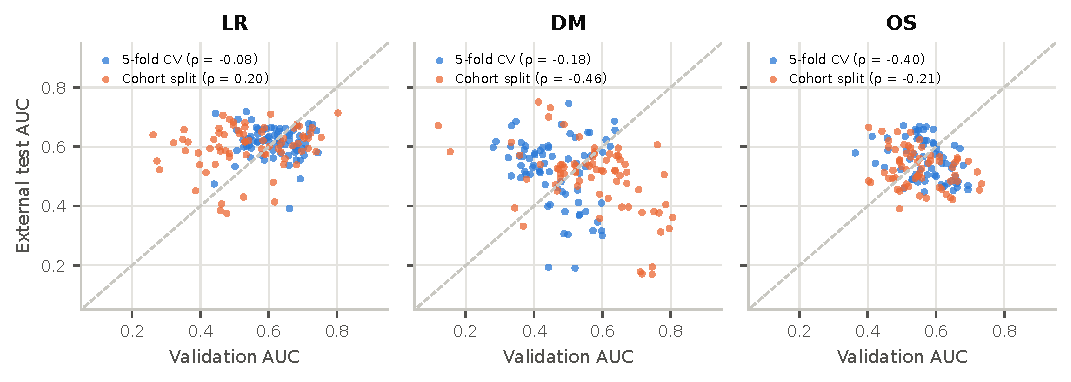
\includegraphics[width=\textwidth]{fig8_val_vs_test.pdf}
\caption{Validation AUC versus external AUC for every GAT configuration under the primary checkpoint rule. The dashed line is the identity. Correlations close to or below zero show that validation performance did not identify configurations that generalise.}\label{fig:valtest}
\end{figure}

\subsection{Sensitivity analysis and attention distribution}
Replacing the lowest-validation-loss checkpoint by the rule of Mateus et al.\ changed the external AUC of the reference configuration by a median of \ruleRefMed{} and at most \ruleRefMax. The configurations chosen on validation changed more, because the rule also altered which configuration ranked first; for DM in cross-validation with imaging alone, for example, the chosen AUC fell from \aucDMCVImgChosen{} to 0.33. The overall conclusions were unaffected (Supplementary Table~S8).

The attention of the GTV read-out node was nearly uniform (Figs.~\ref{fig:folds}b and~\ref{fig:attention}). The final-layer attention to individual supervoxels stayed within about $\pm2\%$ of the per-patient mean, showed no dependence on distance from the GTV, and displayed no visible difference between patients with and without recurrence. Attention maps from these models therefore cannot be interpreted as localising risk.

\begin{figure}[!htb]
\centering
\begin{minipage}[t]{0.47\textwidth}\vspace{0pt}
\panel{a}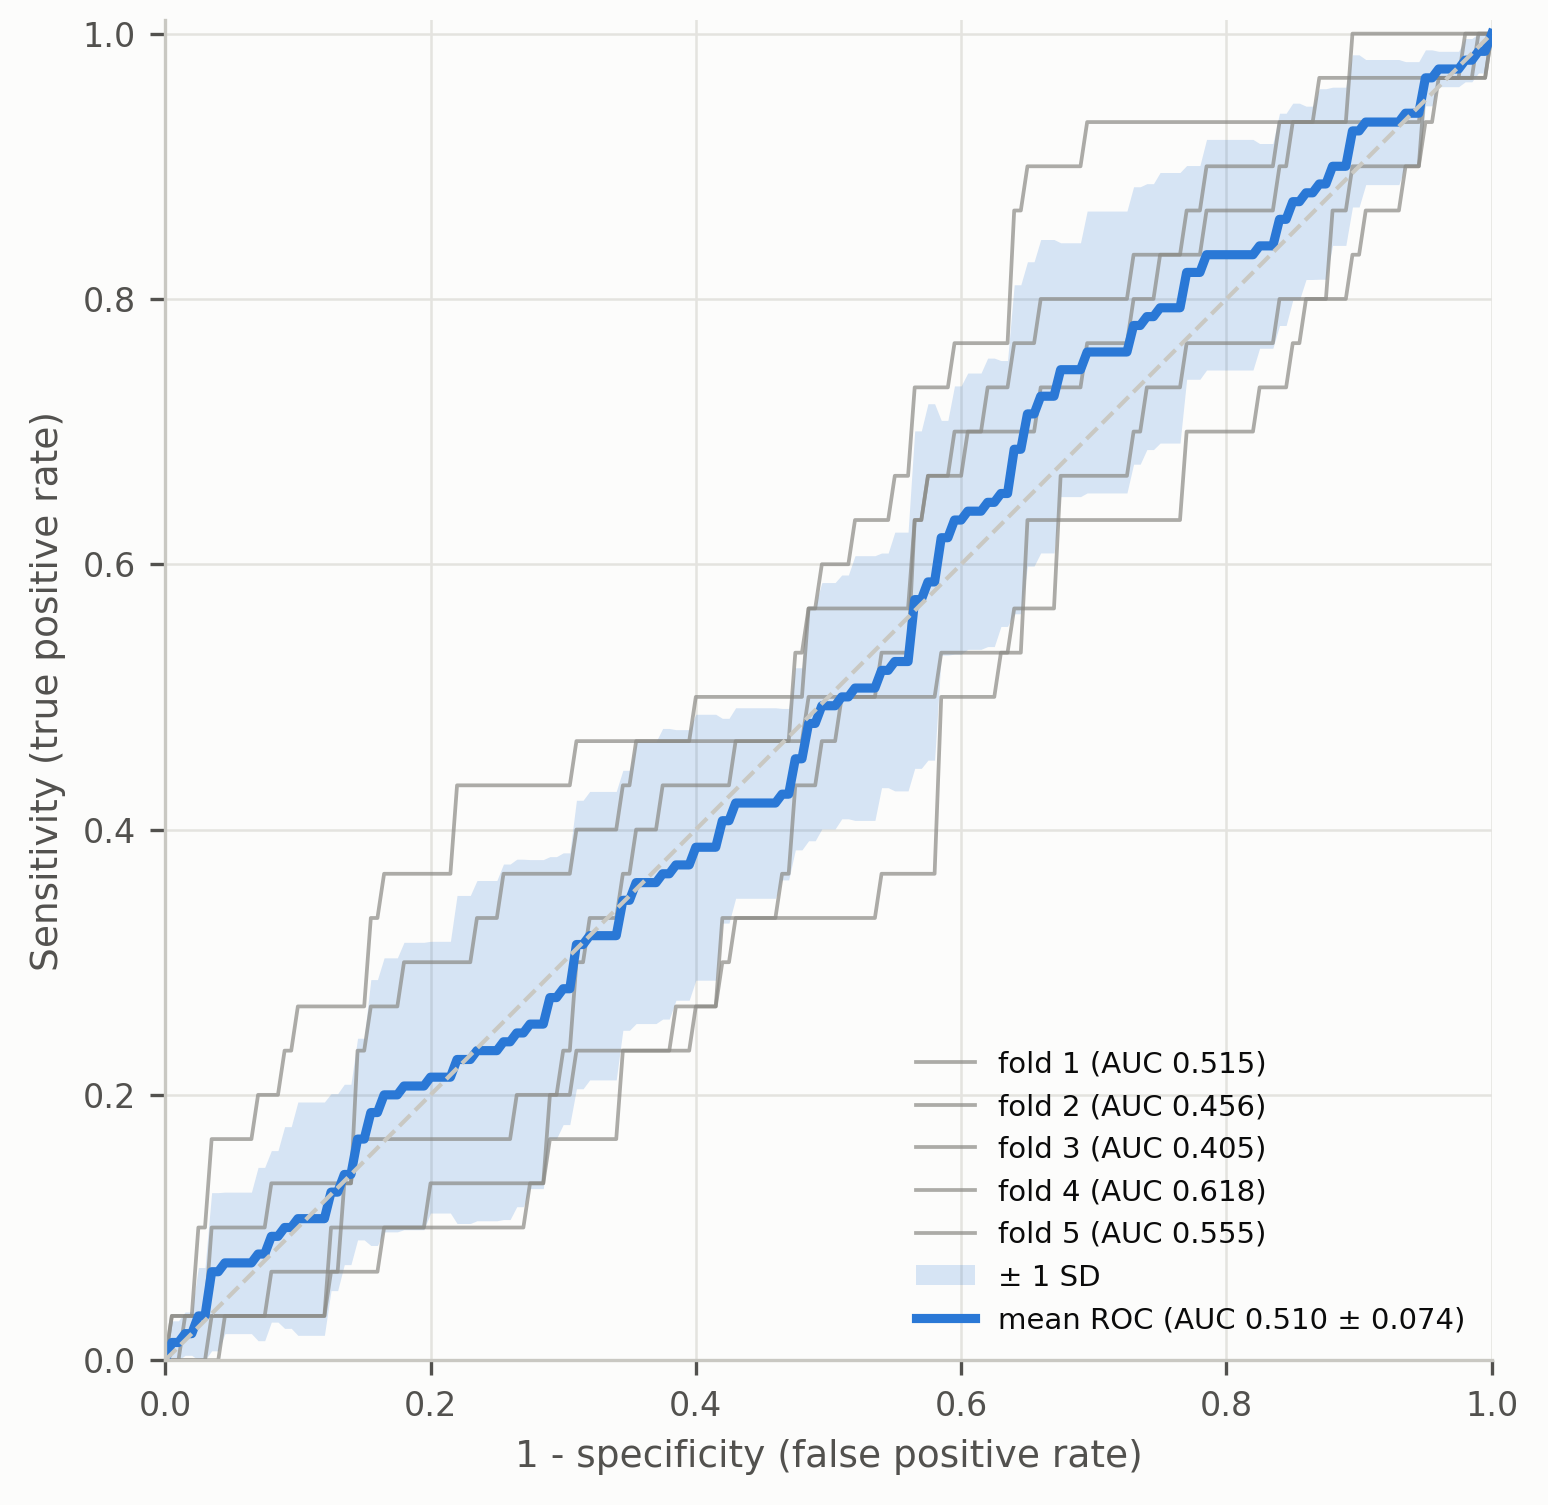
\includegraphics[width=\linewidth]{roc_cv_folds_LR_clean.png}
\end{minipage}\hfill
\begin{minipage}[t]{0.51\textwidth}\vspace{0pt}
\panel{b}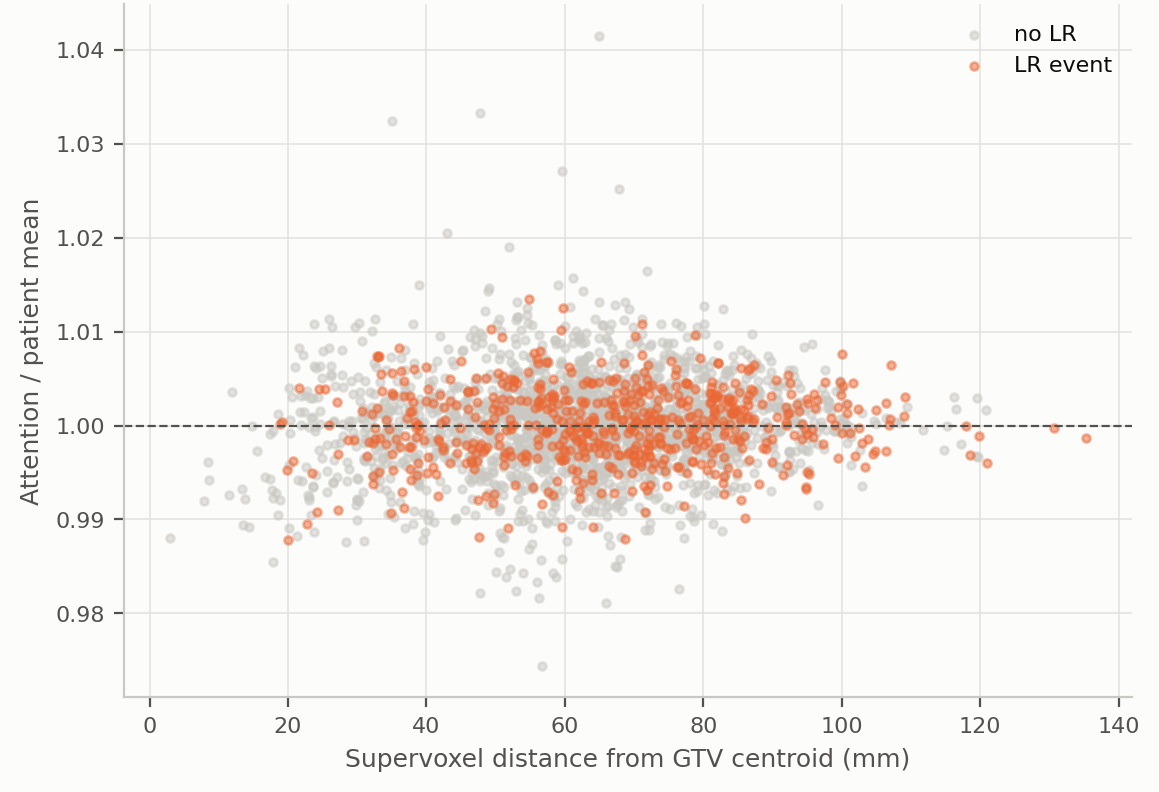
\includegraphics[width=\linewidth]{attention_vs_distance_clean.png}
\end{minipage}
\caption{Fold variability and attention (locoregional recurrence). \textbf{a}~External ROC curves of the five fold models of the configuration chosen in cross-validation, with the mean curve and $\pm1$ standard deviation. \textbf{b}~Final-layer attention of the GTV read-out to each supervoxel, relative to the patient mean, versus distance from the GTV centroid for all external patients (reference configuration, first fold).}\label{fig:folds}
\end{figure}

\begin{figure}[!htb]
\centering
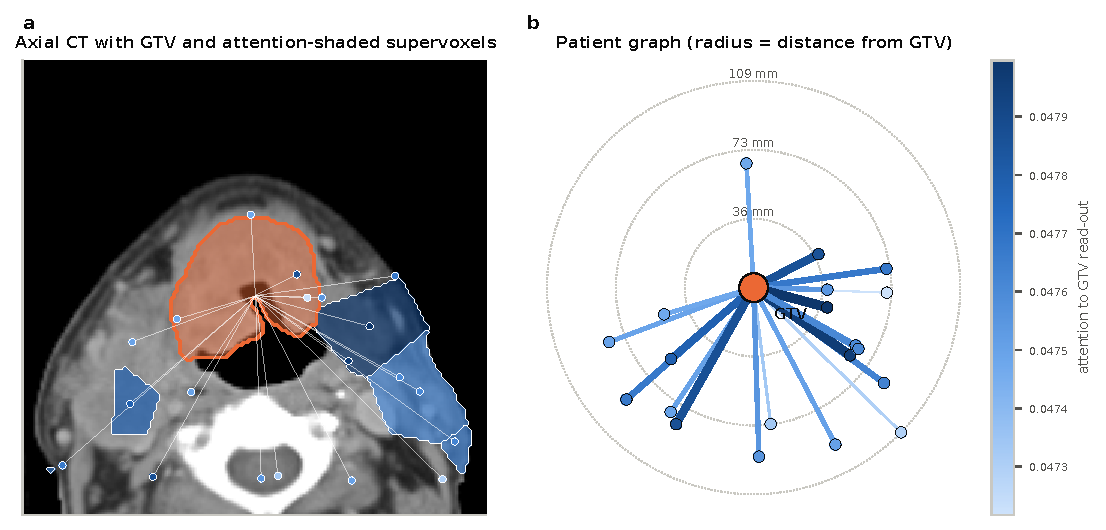
\includegraphics[width=\textwidth]{fig_attention_ct.pdf}
\caption{Attention of the GTV read-out for an external test patient with locoregional recurrence (\attPid, predicted risk \attProb; reference configuration, first fold). \textbf{a}~Axial CT through the GTV (orange) with the intersecting supervoxels shaded by their final-layer attention. \textbf{b}~Patient graph with each supervoxel placed at its in-plane direction and three-dimensional distance from the GTV; edge width and colour encode attention. Attention values range only from \attMin{} to \attMax, close to the uniform value of \attUniform.}\label{fig:attention}
\end{figure}

%% =========================================================================================
\section{Discussion}\label{sec:discussion}

This study benchmarked feature selection and graph topology in spatial radiomic graph attention networks for HNSCC outcome prediction under a validation protocol that permits direct comparison with a published reproducibility study. Graph-based feature selection produced substantially more reproducible node features than LASSO, Boruta and RFE-RF, confirming the stability advantage reported for Graph-FS~\cite{moradmand2025graphfs} in a different setting, namely perturbation of the training data rather than of the radiomic extraction parameters. Neither the selection strategy nor the topology produced a significant improvement in external discrimination over the published RadGraph configuration, and for DM and OS the configurations chosen on validation did not discriminate better than chance. Validation performance, finally, did not identify the configurations that generalised, a methodological observation that extends beyond graph networks.

The feature graph explains why stability and discrimination diverged. Radiomic texture features are highly inter-correlated, so that the Graph-FS graph consists of one large community and a handful of features with distinctive correlation patterns. Label-free Graph-FS repeatedly selects these distinctive features because the community structure barely changes when the training patients change, but nothing guarantees that they carry prognostic information, and in this study they did not. Label-driven selectors behave in the opposite way: in each resample they pick a different member of the large community, which yields unstable selections that are nevertheless broadly interchangeable in predictive terms. The hybrid variant introduced here keeps the redundancy control of the graph but chooses the most outcome-relevant feature within each community; it was both stable (Kuncheva \kunHybLR{} for LR) and among the best LR selectors externally. It therefore appears to be a reasonable default when reproducibility and discrimination must be balanced, although the present evidence is not definitive.

The topology had little influence on LR, and the attention of the read-out node was close to uniform. At this sample size the GAT therefore behaves largely as a smoothed aggregator of peritumoral features rather than learning region-specific weights, which also explains why kNN edges and spatial neighbourhoods made little difference. RadGraph reported informative attention atlases from more than 1500 training patients~\cite{bae2025radgraph}, whereas the development data used here contained \eLRHNPET{} LR events. Nevertheless, the GAT outperformed a random forest on the same GTV features for most selectors when predicting LR, which suggests that the peritumoral tissue contributes some information on locoregional failure beyond the tumour itself.

For LR, the radiomic graph network exceeded the external AUC of the convolutional neural network of Mateus et al.\ in the cohort split (\aucLRCohClinChosen{} versus 0.59 with clinical data) and matched it in cross-validation. Mateus et al.\ described a complete loss of discrimination for LR on MAASTRO, so a peritumoral graph representation may capture information on locoregional failure that a single-slice network does not~\cite{mateus2023}. Conversely, the published network predicted DM (AUC 0.83--0.93) and OS (0.63--0.69) well, whereas the present models did not. Most of this gap is attributable to the development data. The image set available here contained \eDMHNPET{} two-year DM events and \eOSHNPET{} four-year deaths, against \allEvDM{} and \allEvOS{} among all eligible patients of the full collection used by Mateus et al.\ (Supplementary Table~S1), far below common sample-size recommendations for prediction models~\cite{riley2020samplesize}. The development patients were moreover all oropharyngeal while a third of the test patients had laryngeal cancer, a subsite shift that the published network did not face. That a clinical-only random forest was the strongest DM model is consistent with nodal stage being a dominant determinant of distant failure.

The near-zero correlation between validation and external AUC is perhaps the most consequential finding for practice. When more than one hundred configurations are compared on validation folds containing two or three events, the best validation result largely reflects noise, its validation AUC is optimistically biased, and its external performance is unpredictable. Mateus et al.\ observed the same phenomenon for checkpoint selection~\cite{mateus2023}. Studies that compare many architectures or feature sets on small cohorts should therefore fix a reference configuration in advance and report it alongside any data-driven choice, report the distribution of external performance across the whole grid rather than only its maximum, and test differences formally with correction for multiple comparisons, as was done here.

Several limitations apply. The development image set covered only \nHNPETimg{} of the \nHNPETclin{} Canadian patients, was restricted to oropharyngeal cancer and contained fewer than half of the events; the complete collection is required for a fair comparison with Mateus et al.\ and is being obtained. The external DM cohort contained seven events, so that DM results cannot be interpreted beyond their confidence intervals. Stability was assessed across data resamples and centres but not across radiomic extraction settings, unlike in the original Graph-FS study~\cite{moradmand2025graphfs}. The supervoxel stage also leaves room for improvement: because the 50\,mm box extends beyond the skin, a median of 22\% of the supervoxels consisted mostly of air, and the min--max intensity normalisation before SLIC compressed soft tissue into a narrow part of the intensity range; a body mask and a soft-tissue window would make the peritumoral nodes more anatomically meaningful. The GAT hyper-parameters were adopted from RadGraph rather than tuned, and OS reused the LR settings. Binary horizons discard censored patients, and survival formulations could use the data more efficiently. Finally, all selectors retained six features to ensure comparability, and native subset sizes may behave differently.

%% =========================================================================================
\section{Conclusion}\label{sec:conclusion}
Graph-based feature selection made the node features of spatial radiomic graph attention networks markedly more reproducible across folds, resamples and centres, and a graph-guided relevance variant combined this stability with competitive discrimination for locoregional recurrence. With the outcome events available in this study, however, neither feature selection nor graph topology improved external discrimination over the published RadGraph configuration, and validation-based model selection proved unreliable. For locoregional recurrence the radiomic graph network matched or exceeded a published convolutional neural network on the same external cohort. Reproducible feature selection, pre-specified reference configurations and larger, event-rich development cohorts are prerequisites for ranking radiomic graph designs.

%% =========================================================================================
\section*{Declarations}

\paragraph{Supplementary information.}The Supplementary Information contains the data provenance and missing-image analysis, implementation details and hyper-parameters, the complete stability results, the external AUC of every configuration, the checkpoint-rule sensitivity analysis and supplementary figures.

\paragraph{Acknowledgements.}The author thanks the investigators who made the Head-Neck-PET-CT and HN1 collections publicly available through The Cancer Imaging Archive.

\paragraph{Funding.}[To be completed; state ``No funding was received for this study'' if applicable.]

\paragraph{Competing interests.}The author declares no competing interests.

\paragraph{Ethics approval and consent to participate.}This study analysed de-identified, publicly available data from The Cancer Imaging Archive. The original studies obtained institutional ethics approval and informed consent or a waiver, and no additional approval was required for this secondary analysis. [Confirm with the institutional ethics committee.]

\paragraph{Consent for publication.}Not applicable.

\paragraph{Data availability.}The Head-Neck-PET-CT (\url{https://doi.org/10.7937/K9/TCIA.2017.8oje5q00}) and HN1 (\url{https://doi.org/10.7937/tcia.2019.8kap372n}) collections are available from The Cancer Imaging Archive. Patient-level predictions and all result tables are provided with the code.

\paragraph{Code availability.}The complete pipeline, trained model checkpoints, an inference tool and the scripts that generate every table and figure are available at [repository URL to be added].

\paragraph{Author contribution.}The author conceived and designed the study, implemented the software, performed all analyses, interpreted the results and wrote the manuscript.

\bibliographystyle{unsrtnat}
{\small
\bibliography{references}}

\end{document}
